\documentclass[light]{lutbeamer} % change between light and dark for the background
%\documentclass[t]{lutbeamer} % use "t" option for top alignment 
\usepackage{caption}
\usepackage{xcolor}
\captionsetup{labelfont={color=gr},textfont={color=gr}}
\DeclareCaptionLabelFormat{nocolon}{#1 #2}
\captionsetup{labelformat=nocolon}
\usepackage{pgfpages}
\usepackage{amssymb}
\usepackage{amsmath}
\usepackage{tabularx}
\usepackage{array}
\usepackage{adjustbox}
\usepackage{hyperref} % Link
\usepackage{bm}
\usepackage{amsfonts}
\usepackage{algorithmic}
\usepackage{textcomp}
\usepackage{xcolor}
\usepackage{algorithm} 
\usepackage{amsthm} % add this package to use the definition environment

\setbeameroption{hide notes} % Only slides
% \setbeameroption{show only notes} % Only notes
% \setbeameroption{show notes on second screen=right} % Both


% Define the custom color using hexadecimal code
\definecolor{customcolor}{HTML}{123363}

% Define a new block environment with a custom background color and white text
\newenvironment{customblock}{%
    \setbeamercolor{block body}{bg=customcolor,fg=white}%
    \begin{block}%
}{%
    \end{block}%
}


\setdepartment{Data Science and Analytics Thrust, Information Hub}
\institute[HKUSTGZ]{The Hong Kong University of Science and Technology (Guangzhou)}
\author{Mingze Gong}
\title{Spatio-Temporal Forecasting}
\subtitle{Deterministic Graph Neural Networks for Carbon Emissions and Generative Probabilistic Stochastic Differential Equation-based Diffusion for Traffic Flow}
\date{\today}


\begin{document}

% front page
{ % all template changes are local to this group.
\setbeamertemplate{navigation symbols}{}
\begin{frame}<article:0>[plain,noframenumbering]
    \begin{tikzpicture}[remember picture,overlay]
        \node[at=(current page.center)] {
            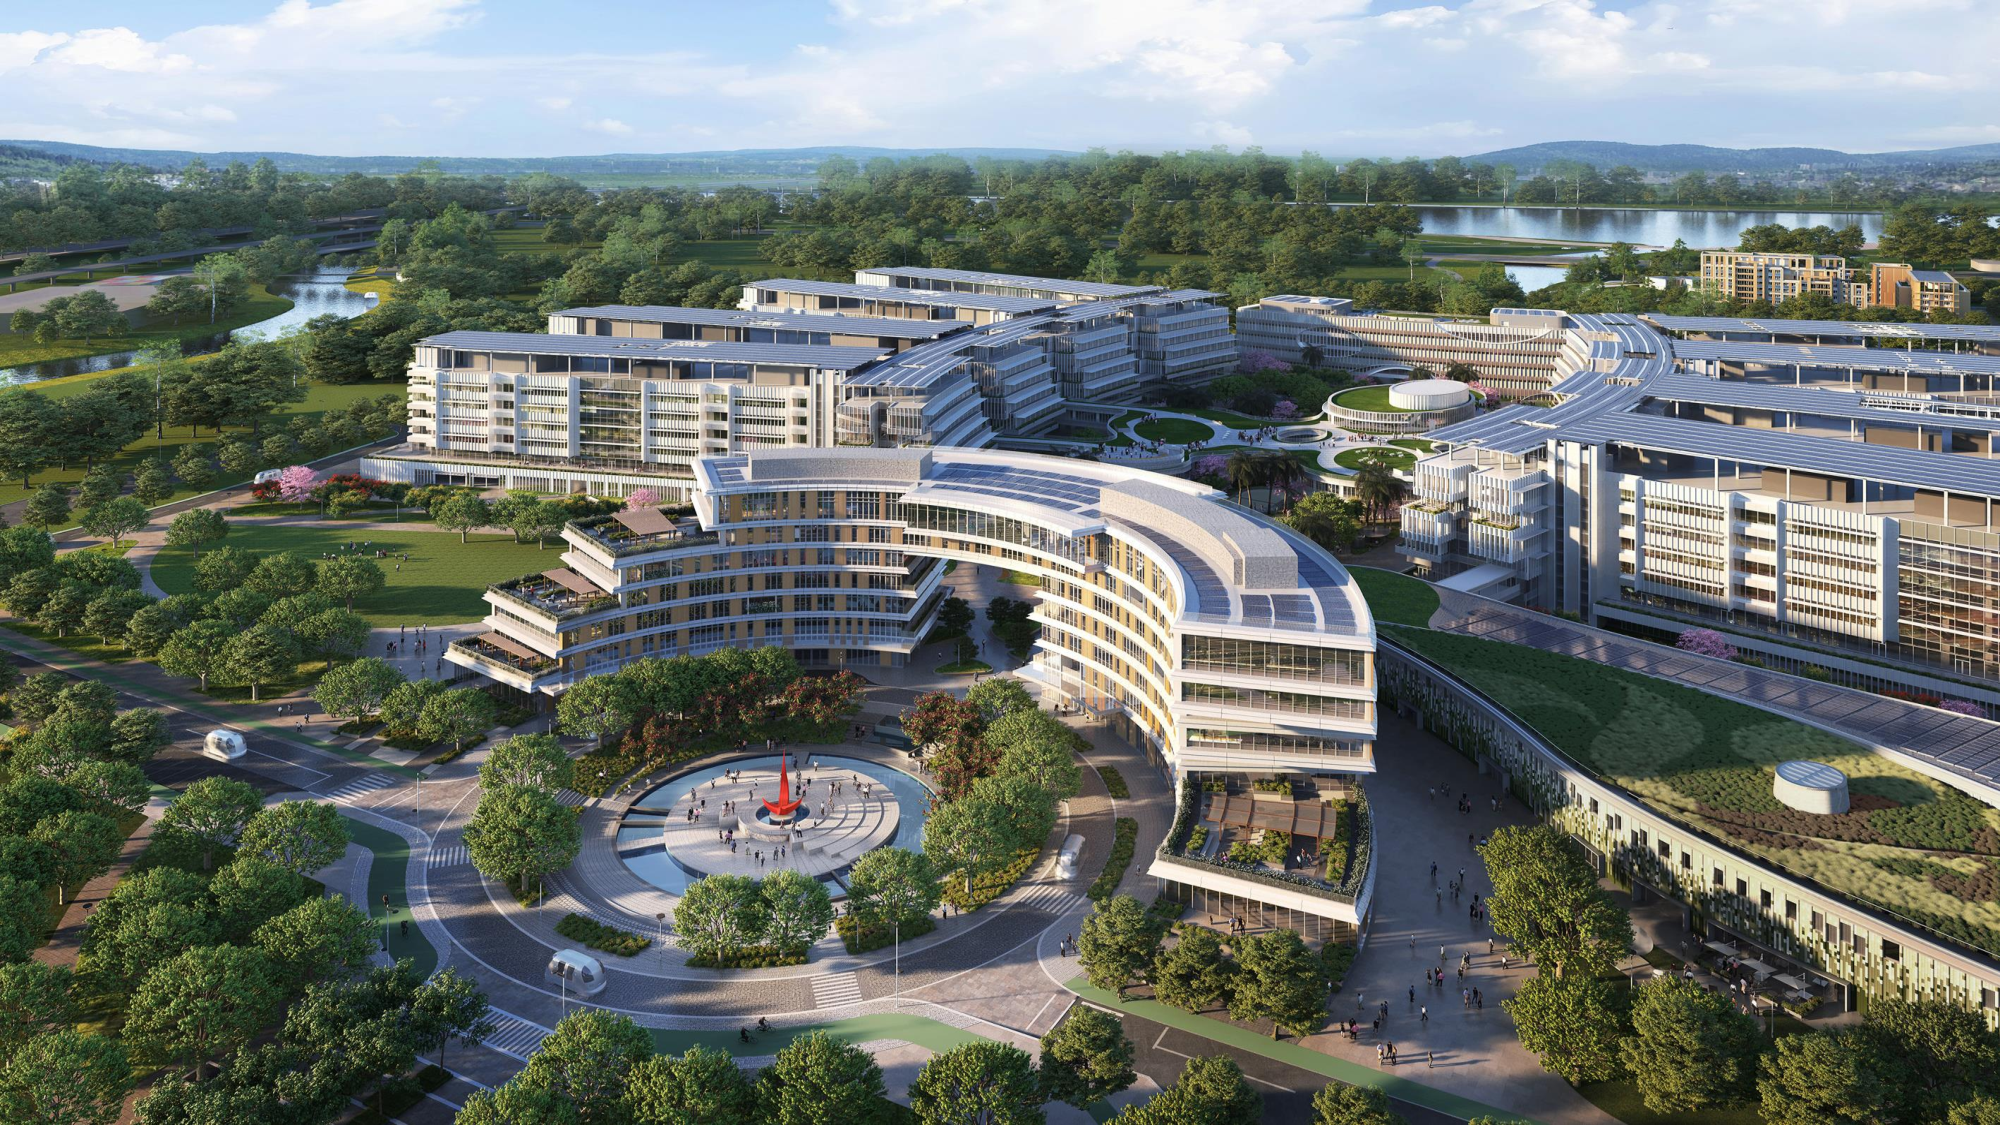
\includegraphics[
                width=\paperwidth,
                height=\paperheight]{figures/GZ Campus.jpeg}
        };
    \end{tikzpicture}
\end{frame}
}

% Outline
\AtBeginSection[]
{
    \begin{frame}[plain,noframenumbering]
        \frametitle{Outline}
        \begin{columns}[T]
            \begin{column}{0.01\textwidth}

            \end{column}
            \begin{column}{0.95\textwidth}
                \tableofcontents[currentsection,
                    %currentsubsection,
                    %hideothersubsections, 
                    %sectionstyle=show/sh ed, 
                    %subsectionstyle=show/shaded%/hide
                ]
            \end{column}
        \end{columns}
    \end{frame}
}

{ % title page
    \begin{frame}[plain]
        \maketitle
        \small
        \par\vskip-0.1em
        {\footnotesize
        \begin{beamercolorbox}[sep=8pt,left]{author}
            \usebeamerfont{author}{Presented by \insertauthor} on \insertdate
        \end{beamercolorbox}%\vskip0.5em
        }
    \end{frame}
}
% % % % % % % % % % % % % % % % % % % % % % % % % % % % % % % % % % % %
\section{Introduction}
\subsection{Acknowledgements}
\begin{frame}
    \frametitle{Acknowledgements}
    \begin{customblock}{}
        I would like to express my sincere gratitude to the committee for your dedication and efforts in joining this event.
        Thank you to my supervisors and mentors for your guidance and help throughout my research journey.
        I appreciate it all.
    \end{customblock}
\end{frame}


\subsection{Research Overview}
\begin{frame}
    \frametitle{Research Overview}
    \framesubtitle{Investigations on Deterministic and Probabilistic Forecasting}
    \begin{columns}
        \begin{column}{0.5\textwidth}
            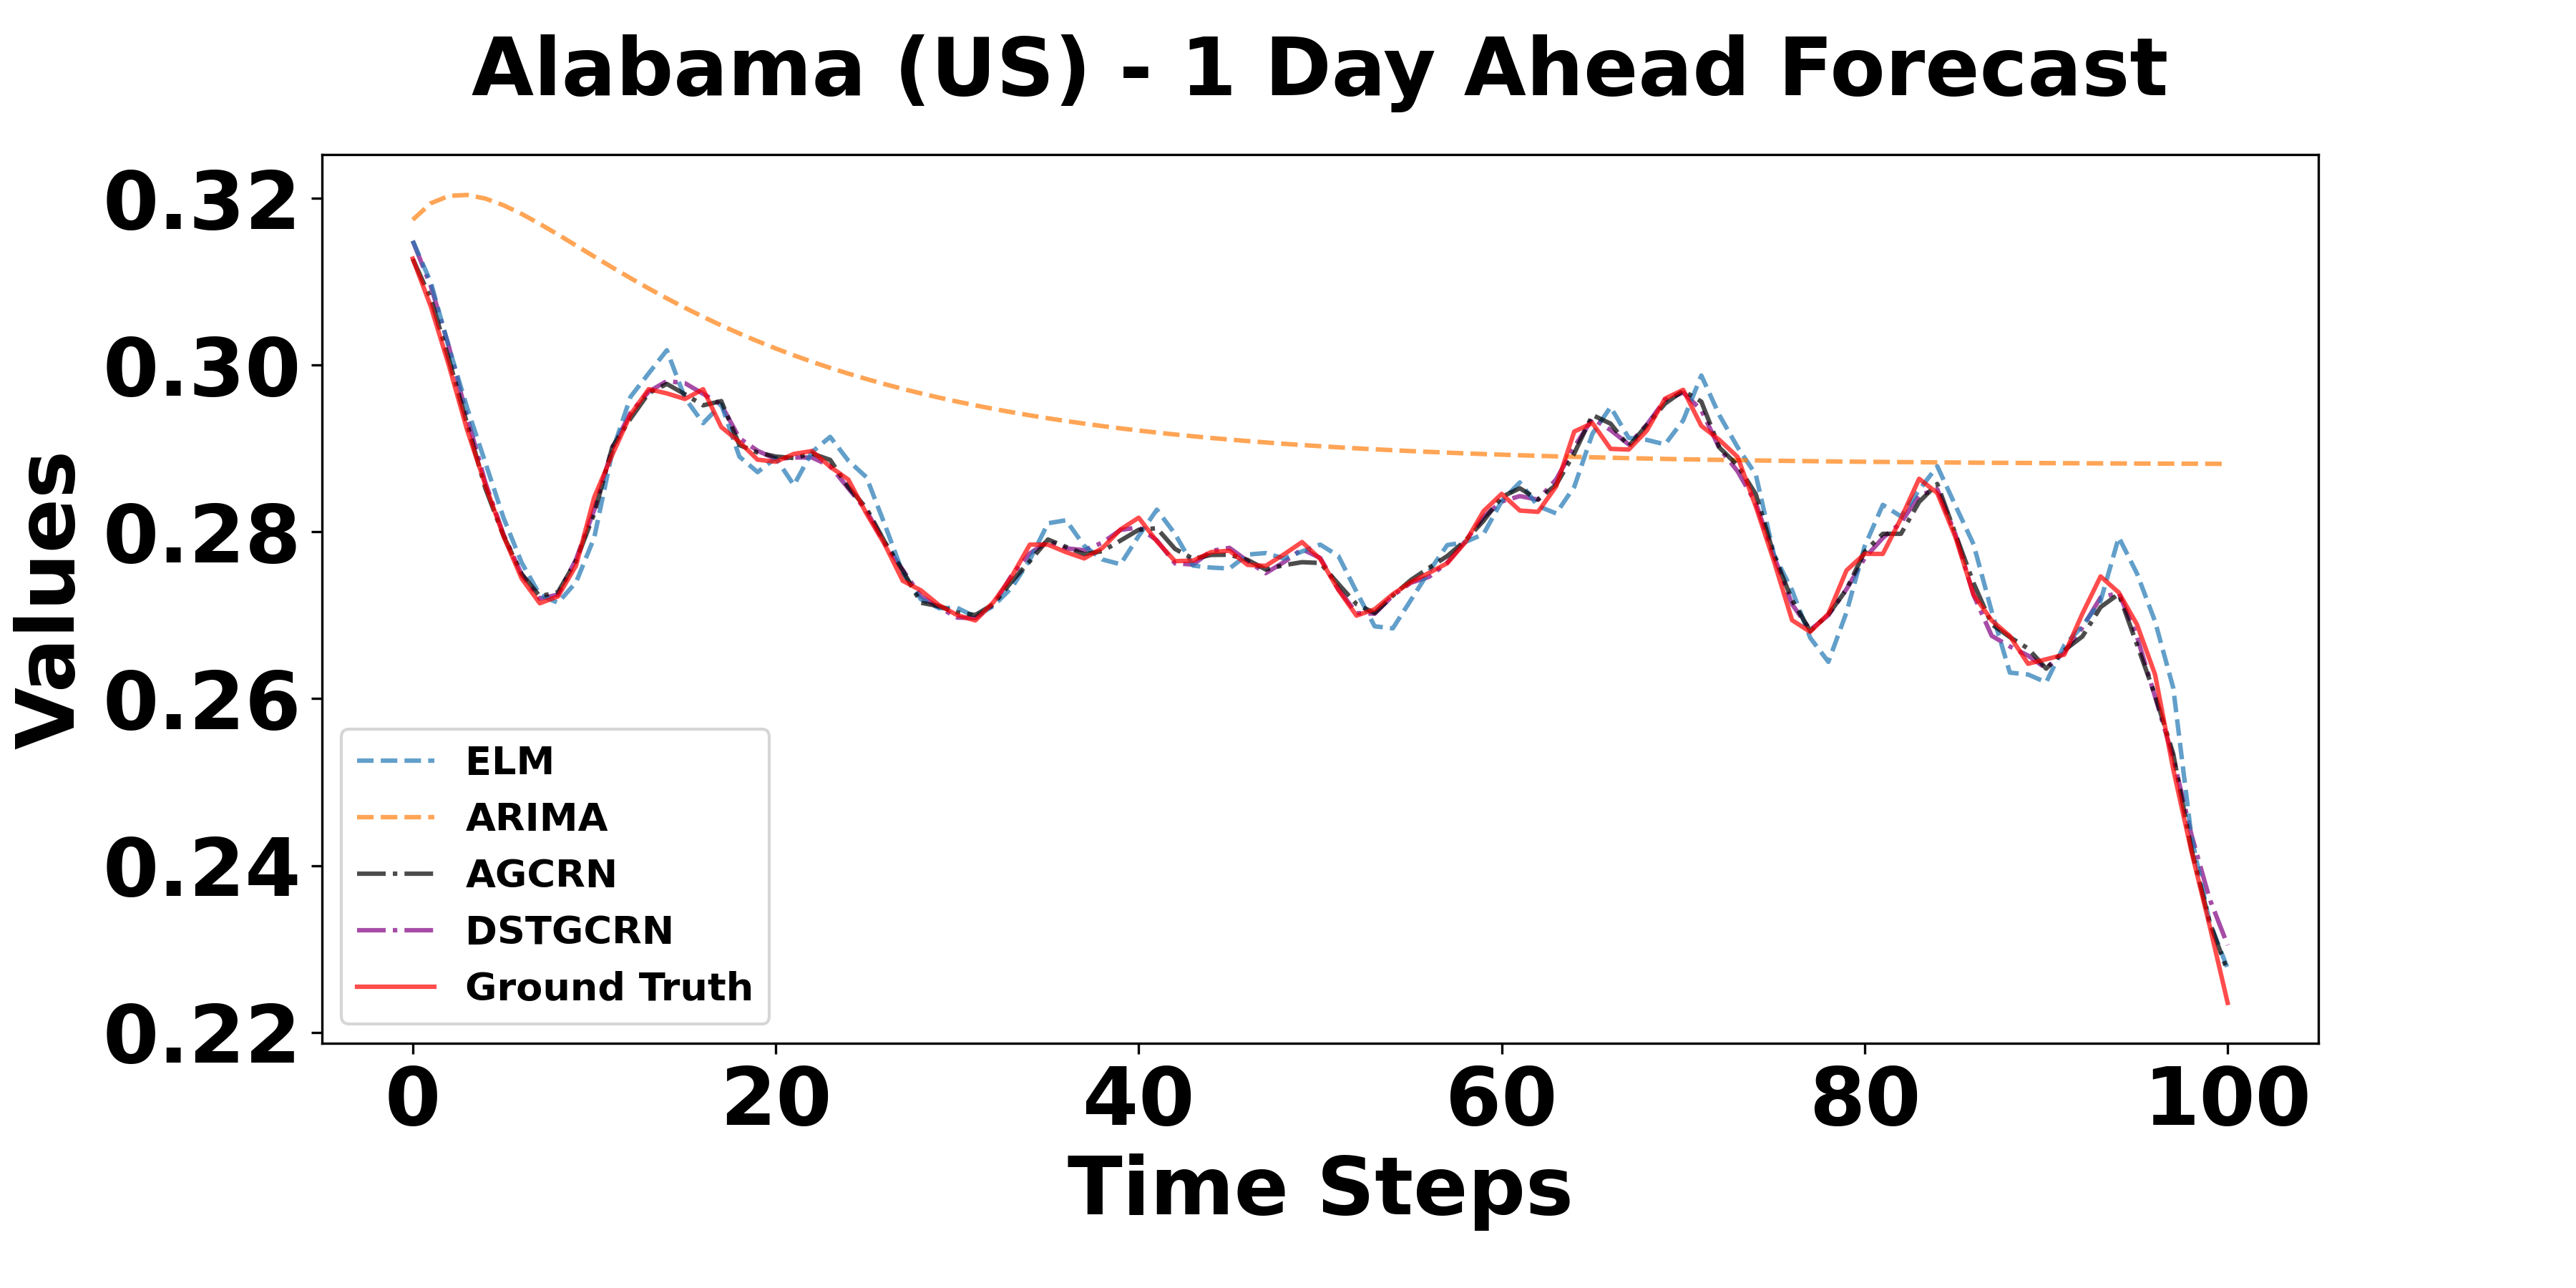
\includegraphics
            [width=\textwidth]{figures/1day_us_0region_modified_new.png}
            \captionof{figure}{A glimpse of forecasts comparison for deterministic carbon emissions forecasting}
        \end{column}
        \begin{column}{0.5\textwidth}
            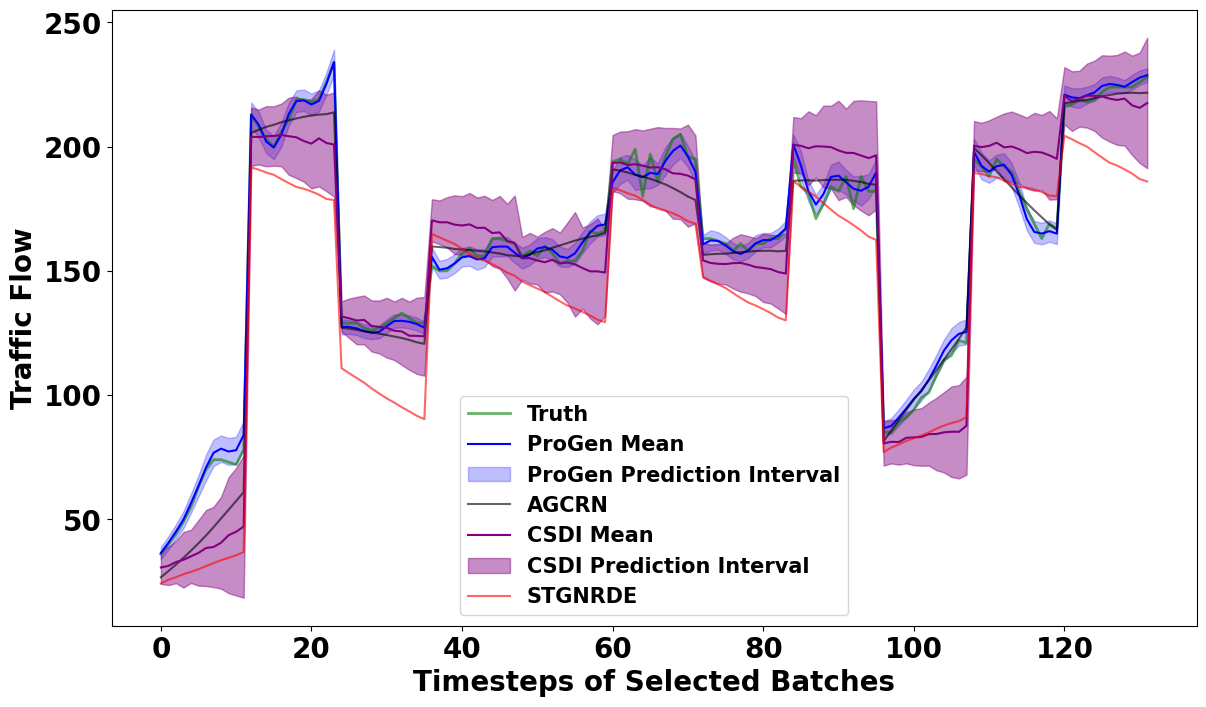
\includegraphics
            [width=\textwidth]{figures/node200_pems04.png}
            \captionof{figure}{A glimpse of forecasts comparison for probabilistic traffic flow forecasting}
        \end{column}
    \end{columns}
\end{frame}

% % % % % % % % % % % % % % % % % % % % % % % % % % % % % % % % % % % %

\section{Deterministic Carbon Emissions Modeling}
\subsection{Introduction to DSTGCRN}
\begin{frame}
    \frametitle{Introduction}
    \framesubtitle{DSTGCRN: Background and Motivation}
    \begin{columns}[T]
        \begin{column}{0.45\textwidth}
            \textbf{Background:}
            \begin{itemize}
                \item Increase in carbon emissions due to fossil fuels and land degradation.
                \item Accurate forecasting is vital to:
                      \begin{itemize}
                          \item Inform sustainable policies.
                          \item Meet reduction targets:
                                \begin{itemize}
                                    \item China: Peak by 2030.
                                    \item US: Reduce 50-52% by 2030.
                                    \item EU: Cut 55% by 2030.
                                \end{itemize}
                      \end{itemize}
            \end{itemize}
        \end{column}
        \begin{column}{0.45\textwidth}
            \textbf{Challenges:}
            \begin{itemize}
                \item Models often overlook non-linear trends and regional dependencies.
                \item Forecasting difficulties:
                      \begin{itemize}
                          \item Variability within regions impacts total emissions.
                          \item Dynamics between regions significantly influence local emissions.
                      \end{itemize}
            \end{itemize}
        \end{column}
    \end{columns}
\end{frame}


\begin{frame}
    \frametitle{Introduction}
    \framesubtitle{DSTGCRN: Motivations and Contributions}
    \begin{columns}[T] % Aligns the top of the content in both columns
        \begin{column}{0.45\textwidth}
            \textbf{Motivations:}
            \begin{itemize}
                \item Overcome limitations of traditional methods in handling complex, dynamic environmental data.
                \item Leverage insights from the success of Graph Neural Networks (GNNs) in sectors such as traffic and energy to enhance spatial-temporal analysis.
            \end{itemize}
        \end{column}
        \begin{column}{0.45\textwidth}
            \textbf{Contributions:}
            \begin{itemize}
                \item Combines Graph Convolutional Networks (GCN) and Recurrent Neural Networks (RNN) to model evolving inter-regional relationships and spatial-temporal dynamics.
                \item Boosts predictive accuracy and offers comprehensive insights to guide environmental policy.
                \item Facilitates informed, real-time policy decisions adapted to specific regional contexts.
            \end{itemize}
        \end{column}
    \end{columns}
\end{frame}

\subsection{Literature Review}

\begin{frame}
    \frametitle{Literature Review}
    \framesubtitle{Statistical and Machine Learning Approaches}
    \begin{itemize}
        \item \textbf{Statistical Methods:}
              \begin{itemize}
                  \item \textbf{ARIMA Models:} Employed for time series forecasting; adjusts for trends and seasonality.
                  \item \textbf{Grey Forecasting Models (GM):} Effective under conditions of limited or incomplete data, applicable in emerging markets.
                  \item \textbf{Hybrid Models:} Combining GM and ARIMA to address non-linear and non-stationary data, enhancing forecast accuracy.
              \end{itemize}
        \item \textbf{Machine Learning Methods:}
              \begin{itemize}
                  \item \textbf{Deep Learning:} Excels in learning complex data patterns, significantly improving prediction capabilities.
                  \item \textbf{Hybrid Approaches:} Integration of neural networks with statistical methods boosts accuracy and reliability.
                  \item \textbf{Regional Variability:} Challenges include accommodating diverse environmental conditions, impacting scalability and model performance.
              \end{itemize}
    \end{itemize}
\end{frame}

\begin{frame}
    \frametitle{Literature Review}
    \framesubtitle{Advancements in Spatial-Temporal Predictions}
    \begin{itemize}
        \item \textbf{Spatial-Temporal Graph Neural Networks (STGNNs):}
              \begin{itemize}
                  \item At the cutting edge for modeling dynamic interdependencies across locations and times, crucial for precise environmental forecasts.
                  \item Adaptive graph structures in these models allow responsiveness to temporal changes, enhancing long-term prediction reliability.
              \end{itemize}
        \item \textbf{Attention Mechanisms:}
              \begin{itemize}
                  \item Prioritize crucial features and time steps, improving focus on significant data and reducing irrelevant noise.
                  \item Demonstrates enhanced detail and accuracy in environmental data analysis, effectively managing spatial and temporal dimensions.
              \end{itemize}
    \end{itemize}
\end{frame}

\subsection{Methodology}

\begin{frame}
    \frametitle{Methodology}
    \framesubtitle{Problem Definitions and Setup}
    \begin{itemize}
        \item \textbf{Multisource Time Series Forecasting:}
              Forecast future values using data from multiple regions on features like temperature and AQI.
              \[
                  \text{Forecast } \bm{Y}_{t+1}, \dots, \bm{Y}_{t+Q} \text{ using } f:\mathbb{R}^{N \times P \times C} \rightarrow \mathbb{R}^{N \times Q}
              \]
              Here, \( \bm{Y}_t \in \mathbb{R}^N \) denotes the output vector at time \( t \), \( P \) is the number of past time steps considered, and \( C \) represents the number of features per step.

        \item \textbf{Regional Carbon Emission Network:}
              Models interdependencies among regions through a graph structure to enhance predictive accuracy by integrating spatial dynamics.
              \[
                  \mathcal{G} = (\mathcal{V}, \mathcal{E}, \bm{A}), \quad \bm{A}_{ij} =
                  \begin{cases}
                      1 & \text{if there is a direct connection between regions } i \text{ and } j, \\
                      0 & \text{otherwise.}
                  \end{cases}
              \]
              Here, \( \mathcal{V} \) are nodes (regions), \( \mathcal{E} \) are edges (connections), and \( \bm{A} \) is the adjacency matrix showing regional connections.
    \end{itemize}
\end{frame}



\begin{frame}
    \frametitle{Methodology}
    \framesubtitle{AGCRN \cite{bai2020}-Core Modeling Approach}
    \begin{itemize}
        \item \textbf{Node Embedding and Graph Convolution:}
              \[
                  \bm{X}'_t = \left(\bm{I}_N + \text{softmax}\left(\text{ReLU}\left(\bm{E} \cdot \bm{E}^\top\right)\right)\right) \bm{X}_t \bm{\Theta}
              \]
              where \(\bm{I}_N\) is the identity matrix, \(\bm{\Theta}\) is the weight matrix.
        \item \textbf{Integration with GRU:}
              \begin{equation}
                  \begin{split}
                      \tilde{\bm A} &= \text{softmax}(\text{ReLU}(\bm E\cdot \bm E^T)) \\
                      {\bm R_t} &= \sigma\left(\tilde{\bm A}[\bm X_t, \bm H_{t-1}]\bm E\bm W_r + \bm E\cdot\bm b_r \right)
                      \\
                      {\bm U_t} &= \sigma\left(\tilde{\bm A}[\bm X_t, \bm H_{t-1}]\bm E\bm W_u + \bm E\cdot\bm b_u \right)
                      \\
                      \hat{\bm H}_t &= \tanh\left(\tilde{\bm A}[\bm X_t, \bm U_t\odot\bm H_{t-1}]\bm E\bm W_h + \bm E\cdot\bm b_h \right)
                      \\
                      \bm H_t &= \bm R_t\odot \bm H_{t-1} + (1-\bm R_t)\odot \hat{\bm H}_t
                  \end{split}
              \end{equation}
    \end{itemize}
\end{frame}


\begin{frame}
    \frametitle{Methodology}
    \framesubtitle{Dynamic Spatial-Temporal Modeling}
    \begin{itemize}
        \item \textbf{Dynamic Embeddings:}
              Generate node embeddings that evolve over time, reflecting changing regional interdependencies. The update mechanism for these embeddings is given by:
              \[
                  \bm{E}_t = \text{DynamicEmbedding}(\bm{\mathcal{X}}_t), \quad \bm{\mathcal{X}}_t \in \mathbb{R}^{P \times N \times C}
              \]
              where \( \bm{\mathcal{X}}_t \) represents the input features across \( P \) past time steps, \( N \) regions, and \( C \) features.

        \item \textbf{Multihead Attention:}
              Applies multihead attention to capture distinct temporal patterns, enhancing the model's predictive accuracy. The mechanism is defined as:
              \[
                  \text{Attention}(\mathbf{Q}, \mathbf{K}, \mathbf{V}) = \text{softmax}\left(\frac{(\bm{\mathcal{X}}''_t \bm{W}_Q)(\bm{\mathcal{X}}''_t \bm{W}_K)^\top}{\sqrt{d_e}}\right)\bm{\mathcal{X}}''_t \bm{W}_V
              \]
              where \(\mathbf{Q}, \mathbf{K}, \mathbf{V}\) are the queries, keys, and values, respectively, transformed by the weight matrices \(\bm{W}_Q, \bm{W}_K, \bm{W}_V\), \( \bm{\mathcal{X}}''_t \) is the processed input, and \( d_e \) denotes the embedding dimension.
    \end{itemize}
\end{frame}


\begin{frame}
    \frametitle{Methodology}
    \framesubtitle{Framework Visualization}
    \begin{figure}
        \centering
        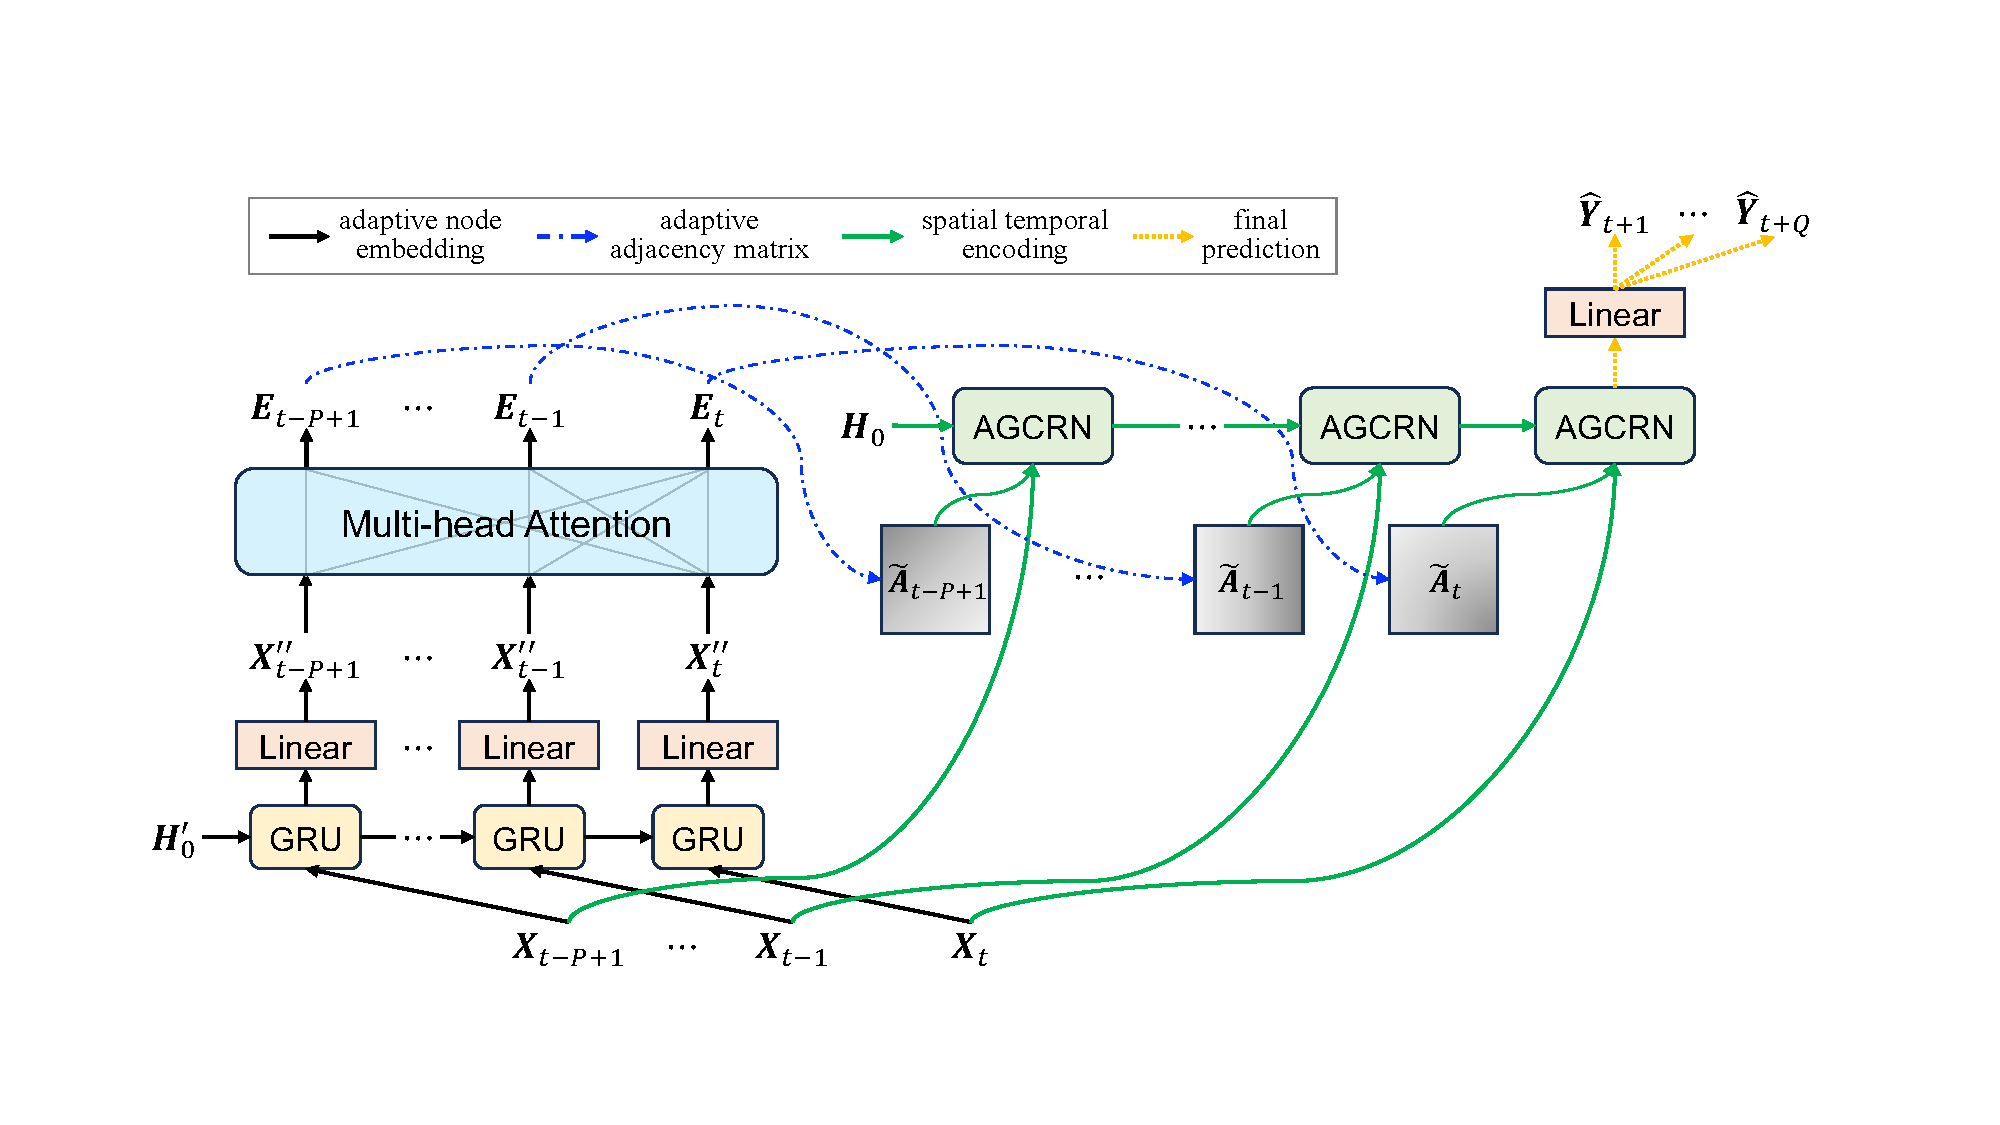
\includegraphics[width=0.8\textwidth]{figures/dstgcrn_framework.pdf}
        \caption{The architecture of the Dynamic Spatial-Temporal Graph Convolutional Recurrent Network (DSTGCRN).}
    \end{figure}
\end{frame}

\subsection{Results}

\begin{frame}
    \frametitle{Results}
    \framesubtitle{Performance Across Datasets}
    \begin{figure}
        \centering
        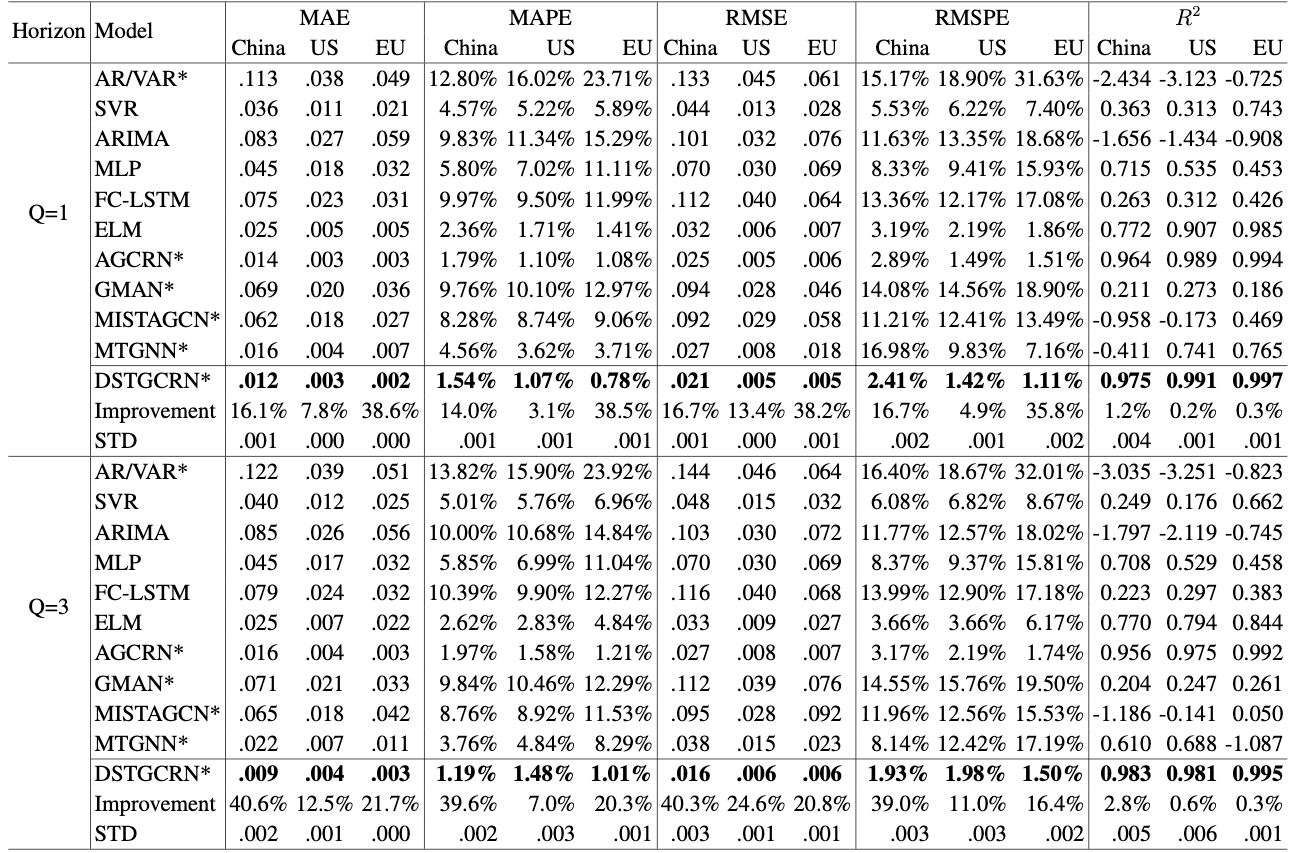
\includegraphics[width=0.6\textwidth]{figures/DSTGCRN_tab_results.png}
        \caption{Comparison of DSTGCRN with baselines after 5 runs on datasets from China, the US, and the EU.}
    \end{figure}
\end{frame}



\begin{frame}
    \frametitle{Results}
    \framesubtitle{Long Term Predictions}

    \begin{figure}
        \centering
        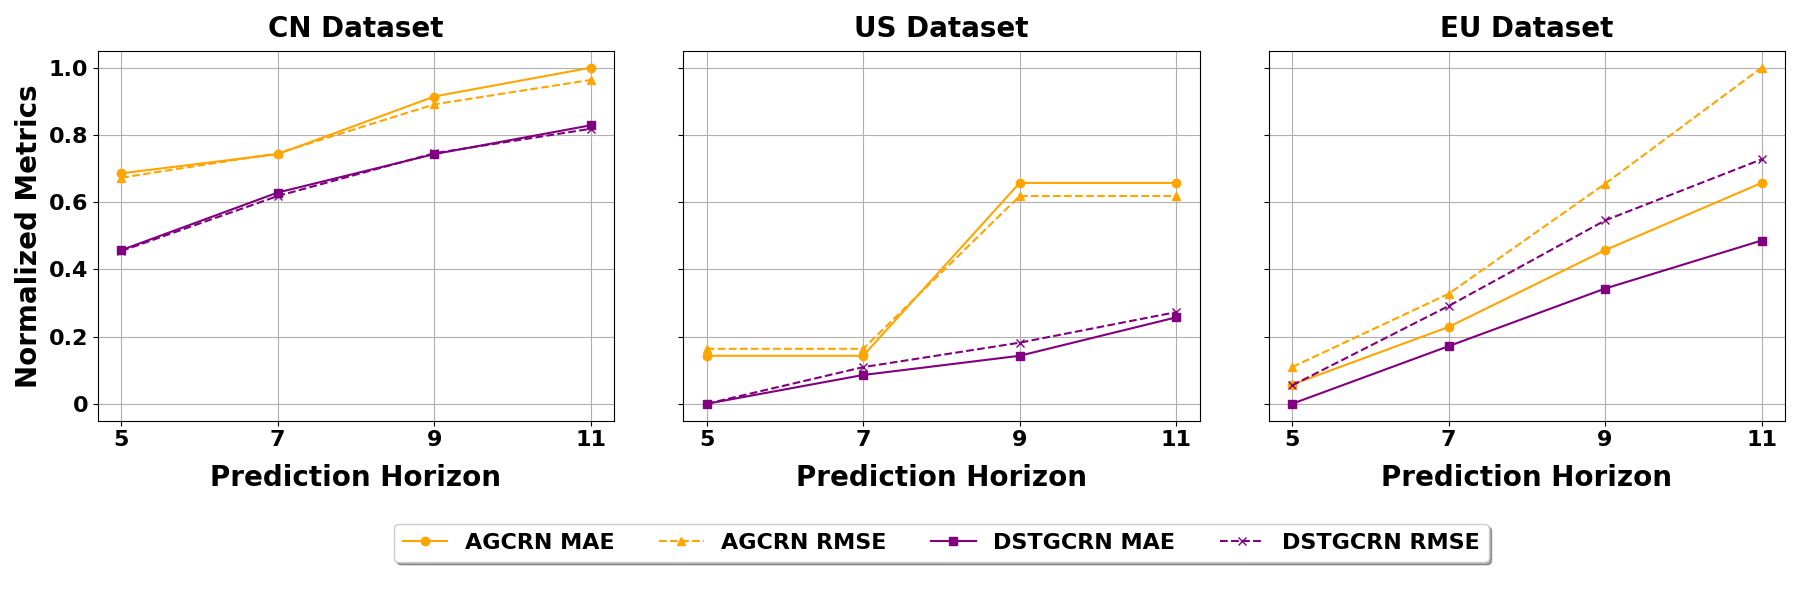
\includegraphics[width=\textwidth]{figures/longer_horizon.png}
        \caption{Performance comparison of AGCRN and DSTGCRN across geographies over longer horizons.}
    \end{figure}

\end{frame}

\begin{frame}
    \frametitle{Results}
    \framesubtitle{Factor Analysis}

    \begin{columns}[T] % Top-aligned columns

        % Left column for the first figure
        \begin{column}{0.48\textwidth}
            \begin{figure}
                \centering
                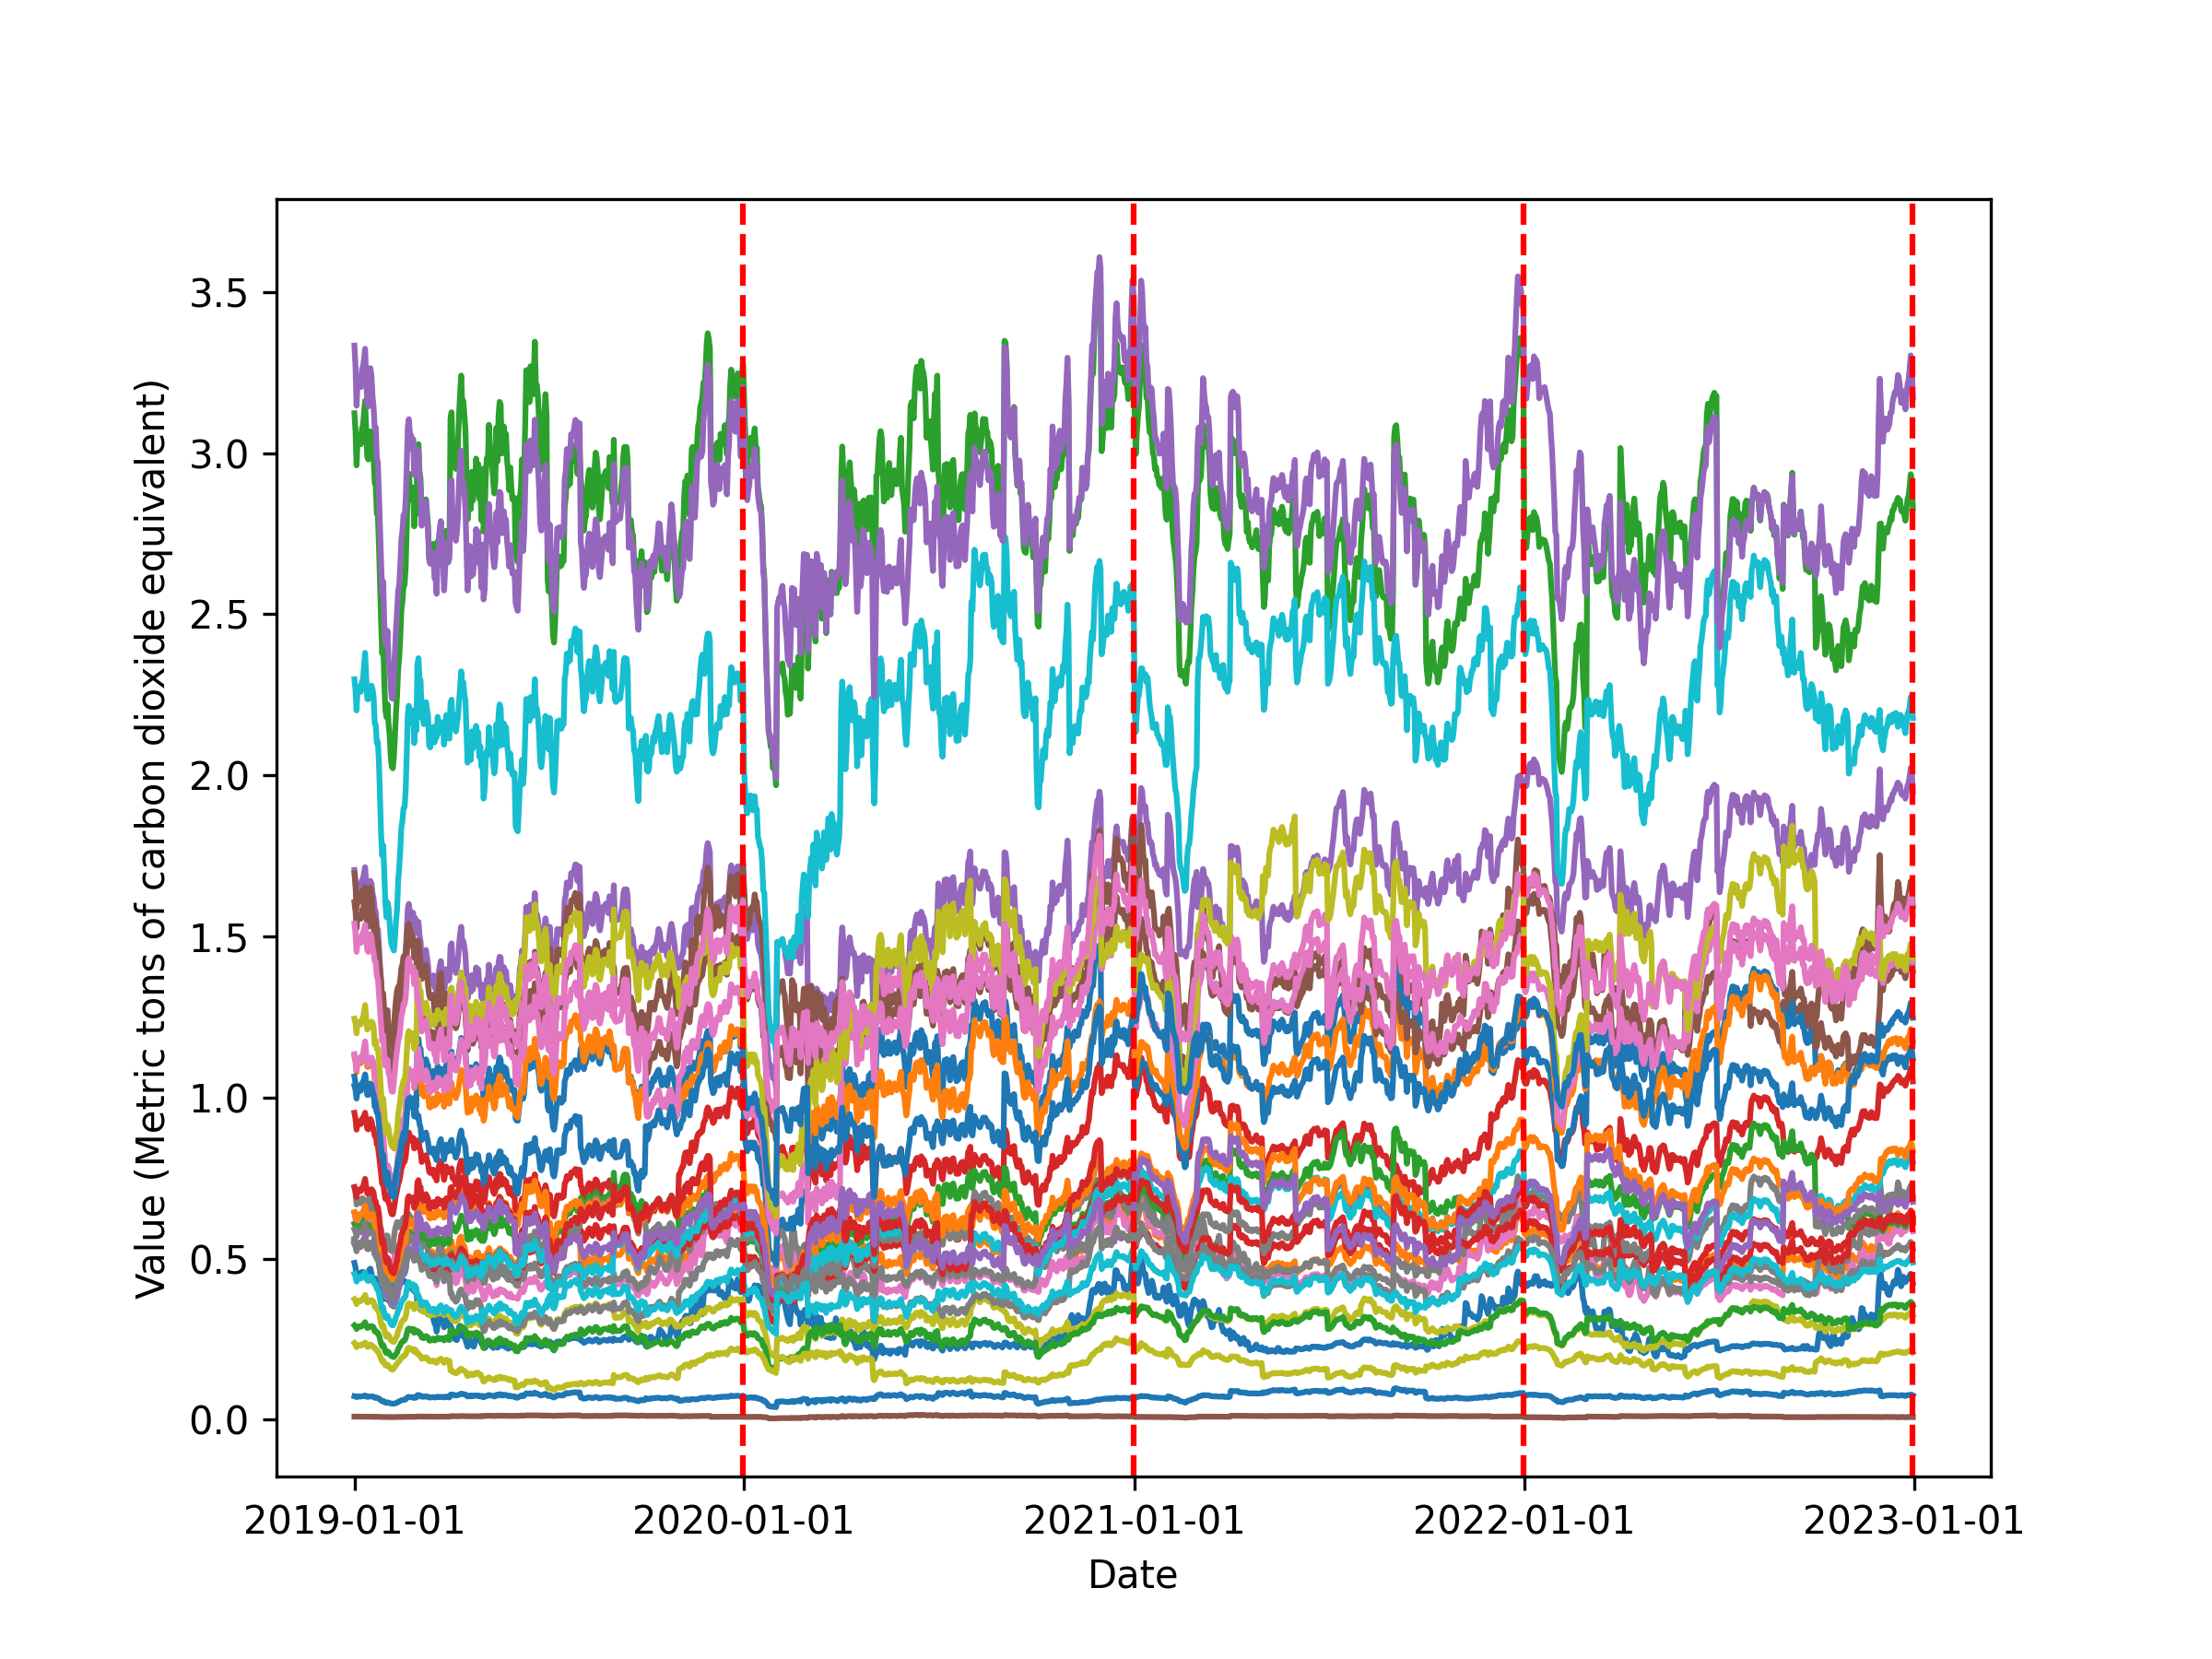
\includegraphics[width=\textwidth]{figures/combined_trend_plot.png}
                \caption{Carbon Emissions Trends from 2019 to 2022 in China.}
            \end{figure}
        \end{column}

        % Right column for the second figure
        \begin{column}{0.48\textwidth}
            \begin{figure}
                \centering
                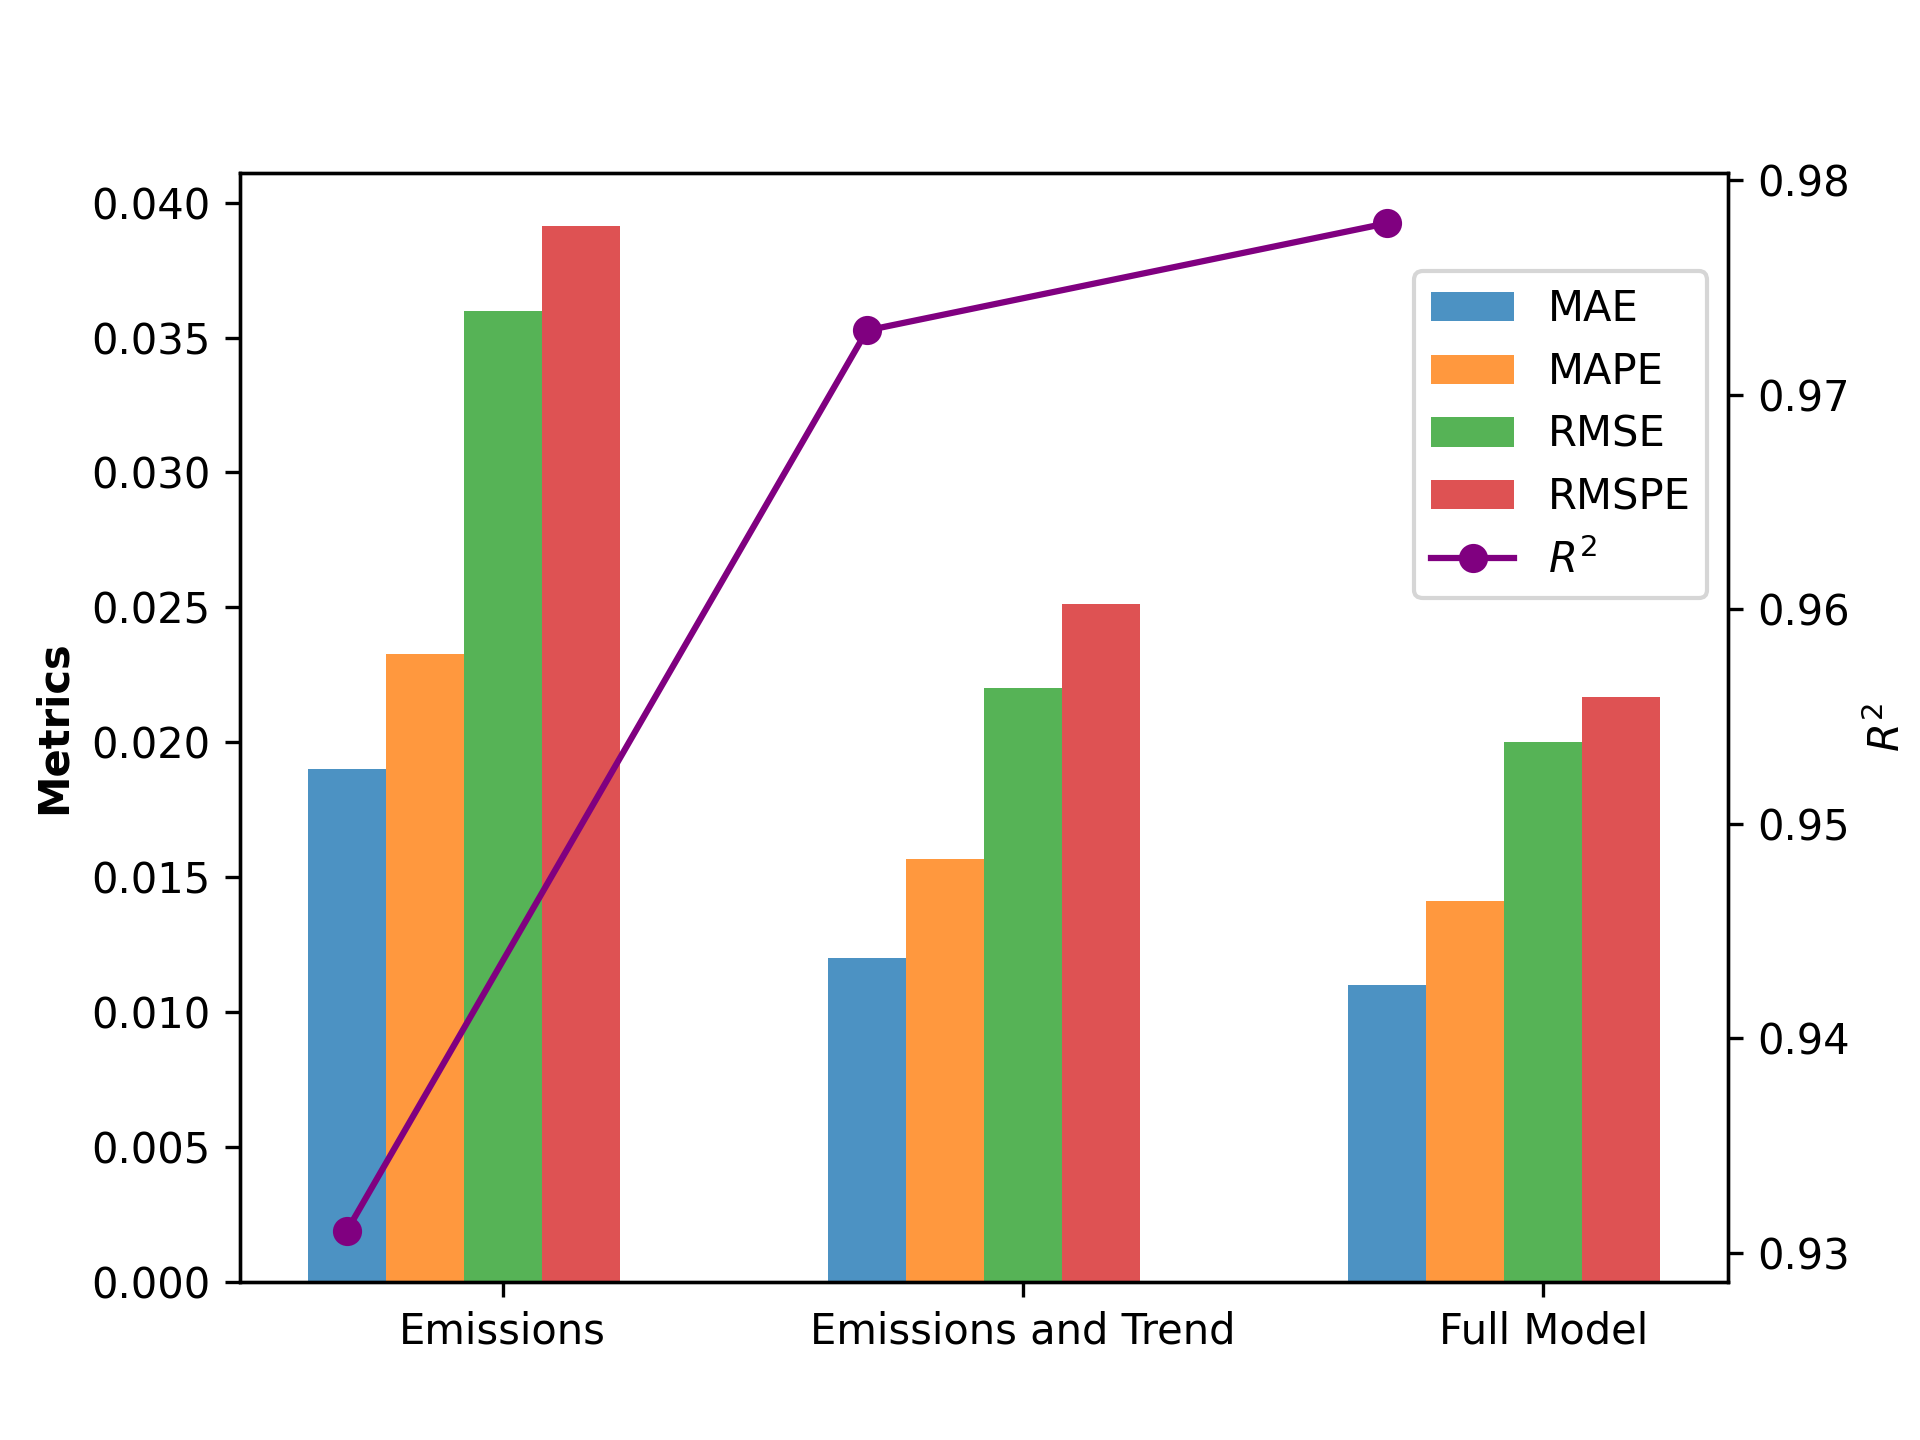
\includegraphics[width=\textwidth]{figures/comparison_feature.png}
                \caption{Performance metrics across three scenarios.}
            \end{figure}
        \end{column}

    \end{columns}
\end{frame}

\begin{frame}
    \frametitle{Results}
    \framesubtitle{Relationship Evolution and Ablation Studies}

    \begin{columns} % Top-aligned columns

        % Left column for the first figure
        \begin{column}{0.48\textwidth}
            \begin{figure}
                \centering
                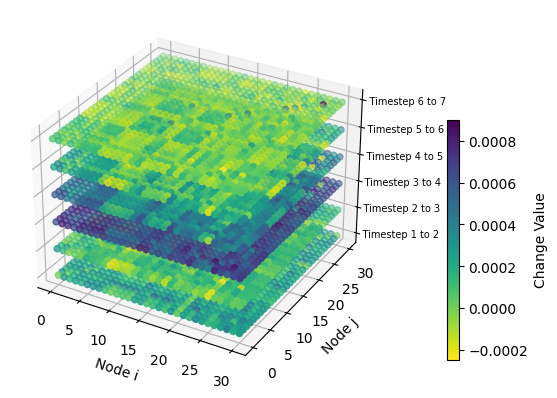
\includegraphics[width=\textwidth]{figures/adj_heatmap_stack.png}
                \caption{Differential Temporal Adjacency Matrix Evolution.}
            \end{figure}
        \end{column}

        % Right column for the second figure
        \begin{column}{0.48\textwidth}
            \begin{figure}
                \centering
                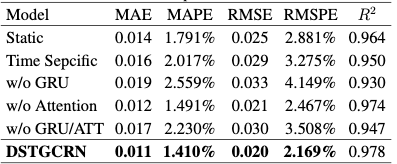
\includegraphics[width=\textwidth]{figures/dstgcrn_ablation.png}
                \caption{Ablation experiments on DSTGCRN.}
            \end{figure}
        \end{column}

    \end{columns}
\end{frame}

\section{Probabilistic Traffic Flow Forecasting}

\subsection{Introduction to ProGen}
\begin{frame}
    \frametitle{Introduction}
    \framesubtitle{Background and Challenges}

    \begin{columns}[T]
        \begin{column}{0.48\textwidth}
            \textbf{Background:}
            \begin{itemize}
                \item Spatial-temporal data exhibits complex spatial dependencies and dynamic temporal evolution.
                \item Conventional forecasting models often provide deterministic outputs, which do not account for data uncertainties.
            \end{itemize}
        \end{column}
        \begin{column}{0.48\textwidth}
            \textbf{Challenges:}
            \begin{itemize}
                \item Modeling spatial-temporal interactions is complex due to their intricate structures.
                \item Traditional deterministic approaches fail to handle the probabilistic nature of real-world data, impairing decision-making.
            \end{itemize}
        \end{column}
    \end{columns}
\end{frame}


\begin{frame}
    \frametitle{Introduction}
    \framesubtitle{Motivation and Contributions}

    \begin{columns}[T]
        \begin{column}{0.48\textwidth}
            \textbf{Motivation:}
            \begin{itemize}
                \item Advances in generative AI, especially diffusion models, offer new avenues for probabilistic forecasting that embrace data uncertainty.
                \item ProGen leverages stochastic differential equations to model data’s continuous-time evolution, improving forecast precision.
            \end{itemize}
        \end{column}
        \begin{column}{0.48\textwidth}
            \textbf{Contributions:}
            \begin{itemize}
                \item \textbf{Conceptual:} Pioneering a generative modeling framework for continuous-time spatial-temporal forecasting.
                \item \textbf{Technical:} Develops a unique denoising approach and custom SDE for improved spatiotemporal correlation handling.
                \item \textbf{Empirical:} Proven enhancements over traditional models validated through rigorous real-world data testing.
            \end{itemize}
        \end{column}
    \end{columns}
\end{frame}


\begin{frame}
    \frametitle{Introduction}
    \framesubtitle{Practical Implementation and Forecasting Implications}

    ProGen's implementation of DSM and SDEs offers several key advantages for spatio-temporal forecasting:
    \begin{itemize}
        \item \textbf{Improved Forecast Accuracy:} By accounting for uncertainty and enabling the model to explore a range of possible futures.
        \item \textbf{Robustness to Noise:} The use of SDEs helps handle the inherent noise and variability in spatio-temporal data effectively.
        \item \textbf{Flexibility in Model Application:} Suitable for various types of spatio-temporal data beyond just traffic or weather, including economic and biological datasets.
    \end{itemize}
    Additionally, the continuous-time approach of ProGen allows for finer temporal resolution in predictions, crucial for dynamic systems monitoring and decision-making.
\end{frame}

\subsection{Literature Review}
\begin{frame}
    \frametitle{Literature Review}
    \framesubtitle{Diffusion Models and Probabilistic Time Series Forecasting}

    \begin{columns}[T]
        \begin{column}{0.48\textwidth}
            \textbf{Diffusion Models:}
            \begin{itemize}
                \item Originated by \citet{ho2020} and \citet{song2021}, using discrete and continuous SDEs to generate data from noise.
                \item Enhanced for conditional generation, aligning outputs with specific attributes.
            \end{itemize}
        \end{column}
        \begin{column}{0.48\textwidth}
            \textbf{Probabilistic Time Series Forecasting:}
            \begin{itemize}
                \item Diffusion models adapted for time series, exemplified by TimeGrad and ScoreGrad, though challenges persist with speed and precision.
                \item ProGen employs a continuous approach, enhancing the capture of spatial and temporal correlations.
            \end{itemize}
        \end{column}
    \end{columns}
\end{frame}

\begin{frame}
    \frametitle{Literature Review}
    \framesubtitle{Spatio-Temporal Forecasting Methods}

    \begin{columns}[T]
        \begin{column}{0.48\textwidth}
            \textbf{Spatio-Temporal Forecasting:}
            \begin{itemize}
                \item Techniques such as AGCRN and DSTAGNN use dynamic graphs; STG-NRDE employs neural rough differential equations.
            \end{itemize}
        \end{column}
        \begin{column}{0.48\textwidth}
            \textbf{Continuity in Time Series:}
            \begin{itemize}
                \item Discrete diffusion models explored probabilistic forecasting but struggled with continuity; ProGen introduces a novel continuous-time method, offering a distinct solution.
            \end{itemize}
        \end{column}
    \end{columns}
\end{frame}


\subsection{Methodology}
\begin{frame}
    \frametitle{Methodology}
    \framesubtitle{Problem Setup}

    Our objective is to forecast future values of a spatio-temporal series based on historical data:
    \begin{itemize}
        \item Define \(\mathcal{D} = \{\mathbf{X_t}\}_{t=1}^T\) where \(\mathbf{X_t} \in \mathbb{R}^{N \times D}\) denotes observations at time \(t\) across \(N\) locations, each with \(D\) features.
        \item Spatial dependencies are modeled through a graph \(\mathcal{G} = (\mathcal{V}, \mathcal{E}, A)\), comprising nodes \(\mathcal{V}\), edges \(\mathcal{E}\), and an adjacency matrix \(A\).
    \end{itemize}
    \vspace{-0.65em}
    \begin{block}{Probabilistic Prediction Task}
        Aim to predict the distribution:
        \[
            q_X (\mathbf{X_{T+1:T+H}} \mid \mathbf{X_{T-L+1:T}}, \mathcal{G}, \mathcal{C})
        \]
        where \(L\) and \(H\) denote the length of the historical window and the forecasting horizon, respectively.
    \end{block}
\end{frame}


\begin{frame}
    \frametitle{Methodology}
    \framesubtitle{Stochastic Differential Equations}

    SDEs provide a framework for modeling continuous-time stochastic processes:
    \begin{equation}
        d\mathbf{X} = f(\mathbf{X}, t)dt + g(\mathbf{X}, t)dW,
    \end{equation}
    where:
    \begin{itemize}
        \item \(\mathbf{X} \in \mathbb{R}^d\) represents the state at time \(t\).
        \item \(f(\mathbf{X}, t)\) is the drift function, dictating deterministic dynamics.
        \item \(g(\mathbf{X}, t)\) is the diffusion function, modeling stochastic effects.
        \item \(dW\) denotes differential Brownian motion.
    \end{itemize}
\end{frame}

\begin{frame}
    \frametitle{Methodology}
    \framesubtitle{Reverse Stochastic Differential Equations}

    Reverse SDEs describe how to denoise data back to its original distribution:
    \begin{equation}
        d\mathbf{X} = \left[f(\mathbf{X}, t) - g^2(\mathbf{X}, t)\nabla_X \log p_t(\mathbf{X})\right]dt + g(\mathbf{X}, t)d\bar{W},
    \end{equation}
    \begin{itemize}
        \item The score function \(\nabla_X \log p_t(\mathbf{X})\) guides the denoising process.
        \item \(\bar{W}\) is the reverse Wiener process, introducing reverse dynamics.
    \end{itemize}
\end{frame}

\begin{frame}
    \frametitle{Methodology}
    \framesubtitle{Denoising Score Matching (DSM)}

    DSM optimizes the match between the gradients of the log probabilities (scores) of the model and data distributions through the diffusion process:
    \begin{equation}
        \mathcal{L}(\theta) = \mathbb{E}_{t \sim \text{Uniform}(0, K)} \mathbb{E}_{X \sim p_{\text{data}}} [\|\nabla_X \log q_{\theta}(\mathbf{X^t} | t) - \nabla_X \log p_{\text{data}}(\mathbf{X^t} | t)\|^2]
    \end{equation}
    where:
    \begin{itemize}
        \item \( q_{\theta}(\mathbf{X^t} | t) \) and \( p_{\text{data}}(\mathbf{X^t} | t) \) are the model and data distributions at diffusion timestep \(t\), respectively.
        \item \( \nabla_X \log \) represents the gradient of the log probability.
        \item \( \theta \) denotes the model parameters optimized during training.
    \end{itemize}
\end{frame}



\begin{frame}
    \frametitle{Methodology}
    \framesubtitle{Overview of ProGen Framework}

    ProGen combines a forward diffusion process with a reverse prediction process:
    \begin{itemize}
        \item \textbf{Forward Diffusion:} Transforms training data into a Gaussian state while training a score model.
        \item \textbf{Reverse Prediction:} Iteratively denoises to generate predictions, guided by the score model.
    \end{itemize}

    \begin{figure}[ht]
        \centering
        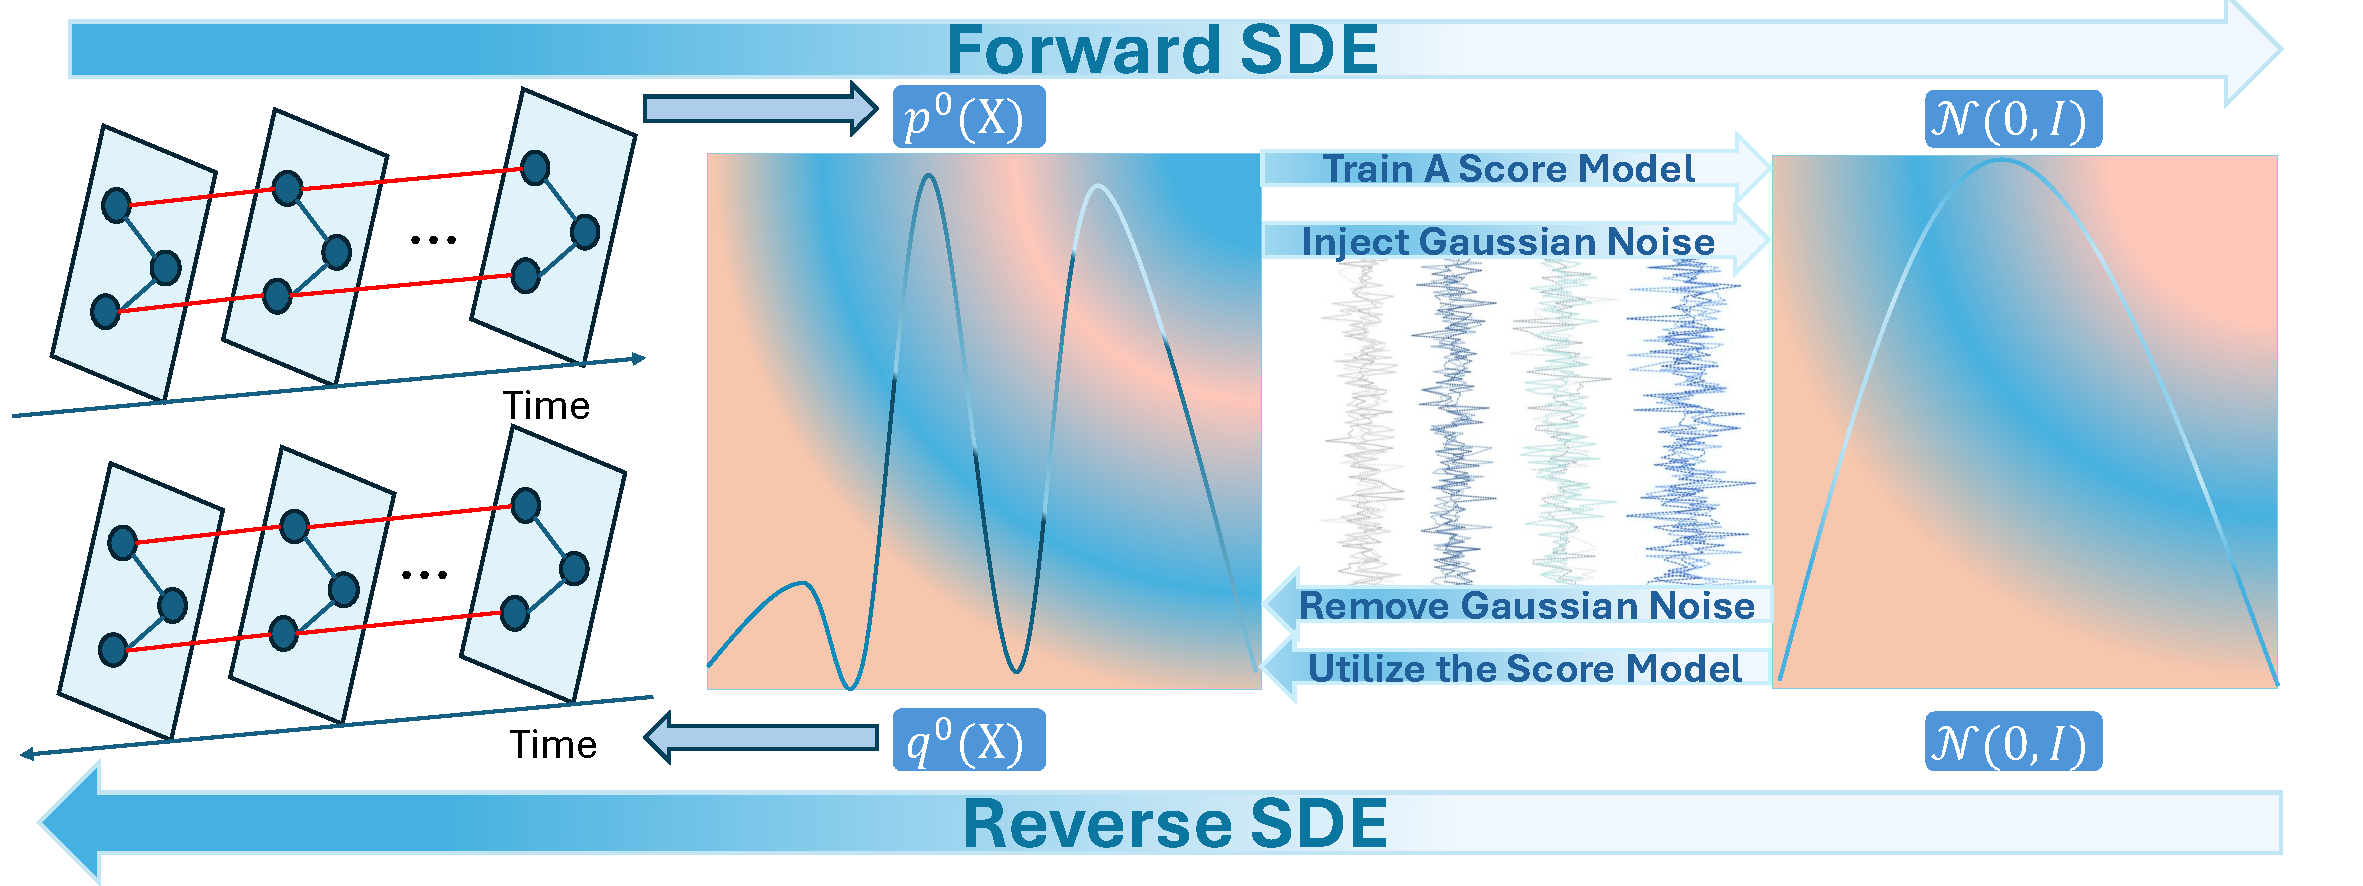
\includegraphics[width=0.7\textwidth]{figures/ProGen_framework_new.pdf}
        \caption{Overview of the two primary processes in ProGen.}
        \label{fig:framework}
    \end{figure}

\end{frame}

\begin{frame}
    \frametitle{Methodology}
    \framesubtitle{Forward Diffusion Process}

    The forward diffusion process incrementally transforms the data points into Gaussian noise:
    \begin{equation}
        \mathbf{\tilde{X}^t_{F}} = \mu(\mathbf{X_{F}}, t, \beta_0, \beta_1) + \sigma(\mathbf{X_{F}}, t, \beta_0, \beta_1) \times Z,
    \end{equation}
    where \(\mu\) and \(\sigma\) are functions that determine the mean and standard deviation at each time step \(t\). \\~\\

    This method trains the model to simulate transitions from actual data distributions to a noise state, aiding in understanding the underlying data dynamics.
\end{frame}


\begin{frame}
    \frametitle{Methodology}
    \framesubtitle{Training the Denoising Score Model}

    Training is focused on minimizing the discrepancy between the estimated and true gradients of the data:
    \begin{equation}
        \begin{aligned}
            \mathcal{L}(\theta) & = \mathbb{E}_{t} \left\{ \lambda(t) \mathbb{E}_{\mathbf{X}_{F}^0, \mathbf{X_H}} \left[ \mathbb{E}_{\tilde{\mathbf{X}}_{F}^t | \mathbf{X}_{F}^0, \mathbf{X_H}} \right. \right.                                                                  \\
                                & \quad \left. \left. \left\| s_\theta(\tilde{\mathbf{X}}_{F}^t, \mathbf{X_H}, \mathcal{G}, t, \mathbf{P_H}) - \nabla_{\tilde{\mathbf{X}}_{F}^t} \log p(\tilde{\mathbf{X}}_{F}^t | \mathbf{X}_{F}^0, \mathbf{X_H}) \right\|_2^2 \right] \right\}
        \end{aligned}
        \label{eq:loss}
    \end{equation}
    This loss function aims to align the model's score estimates with actual distribution changes, thereby enhancing prediction accuracy.
\end{frame}

\begin{frame}
    \frametitle{Methodology}
    \framesubtitle{Model Architecture}
    \vspace{-1em}
    \begin{figure}[ht]
        \centering
        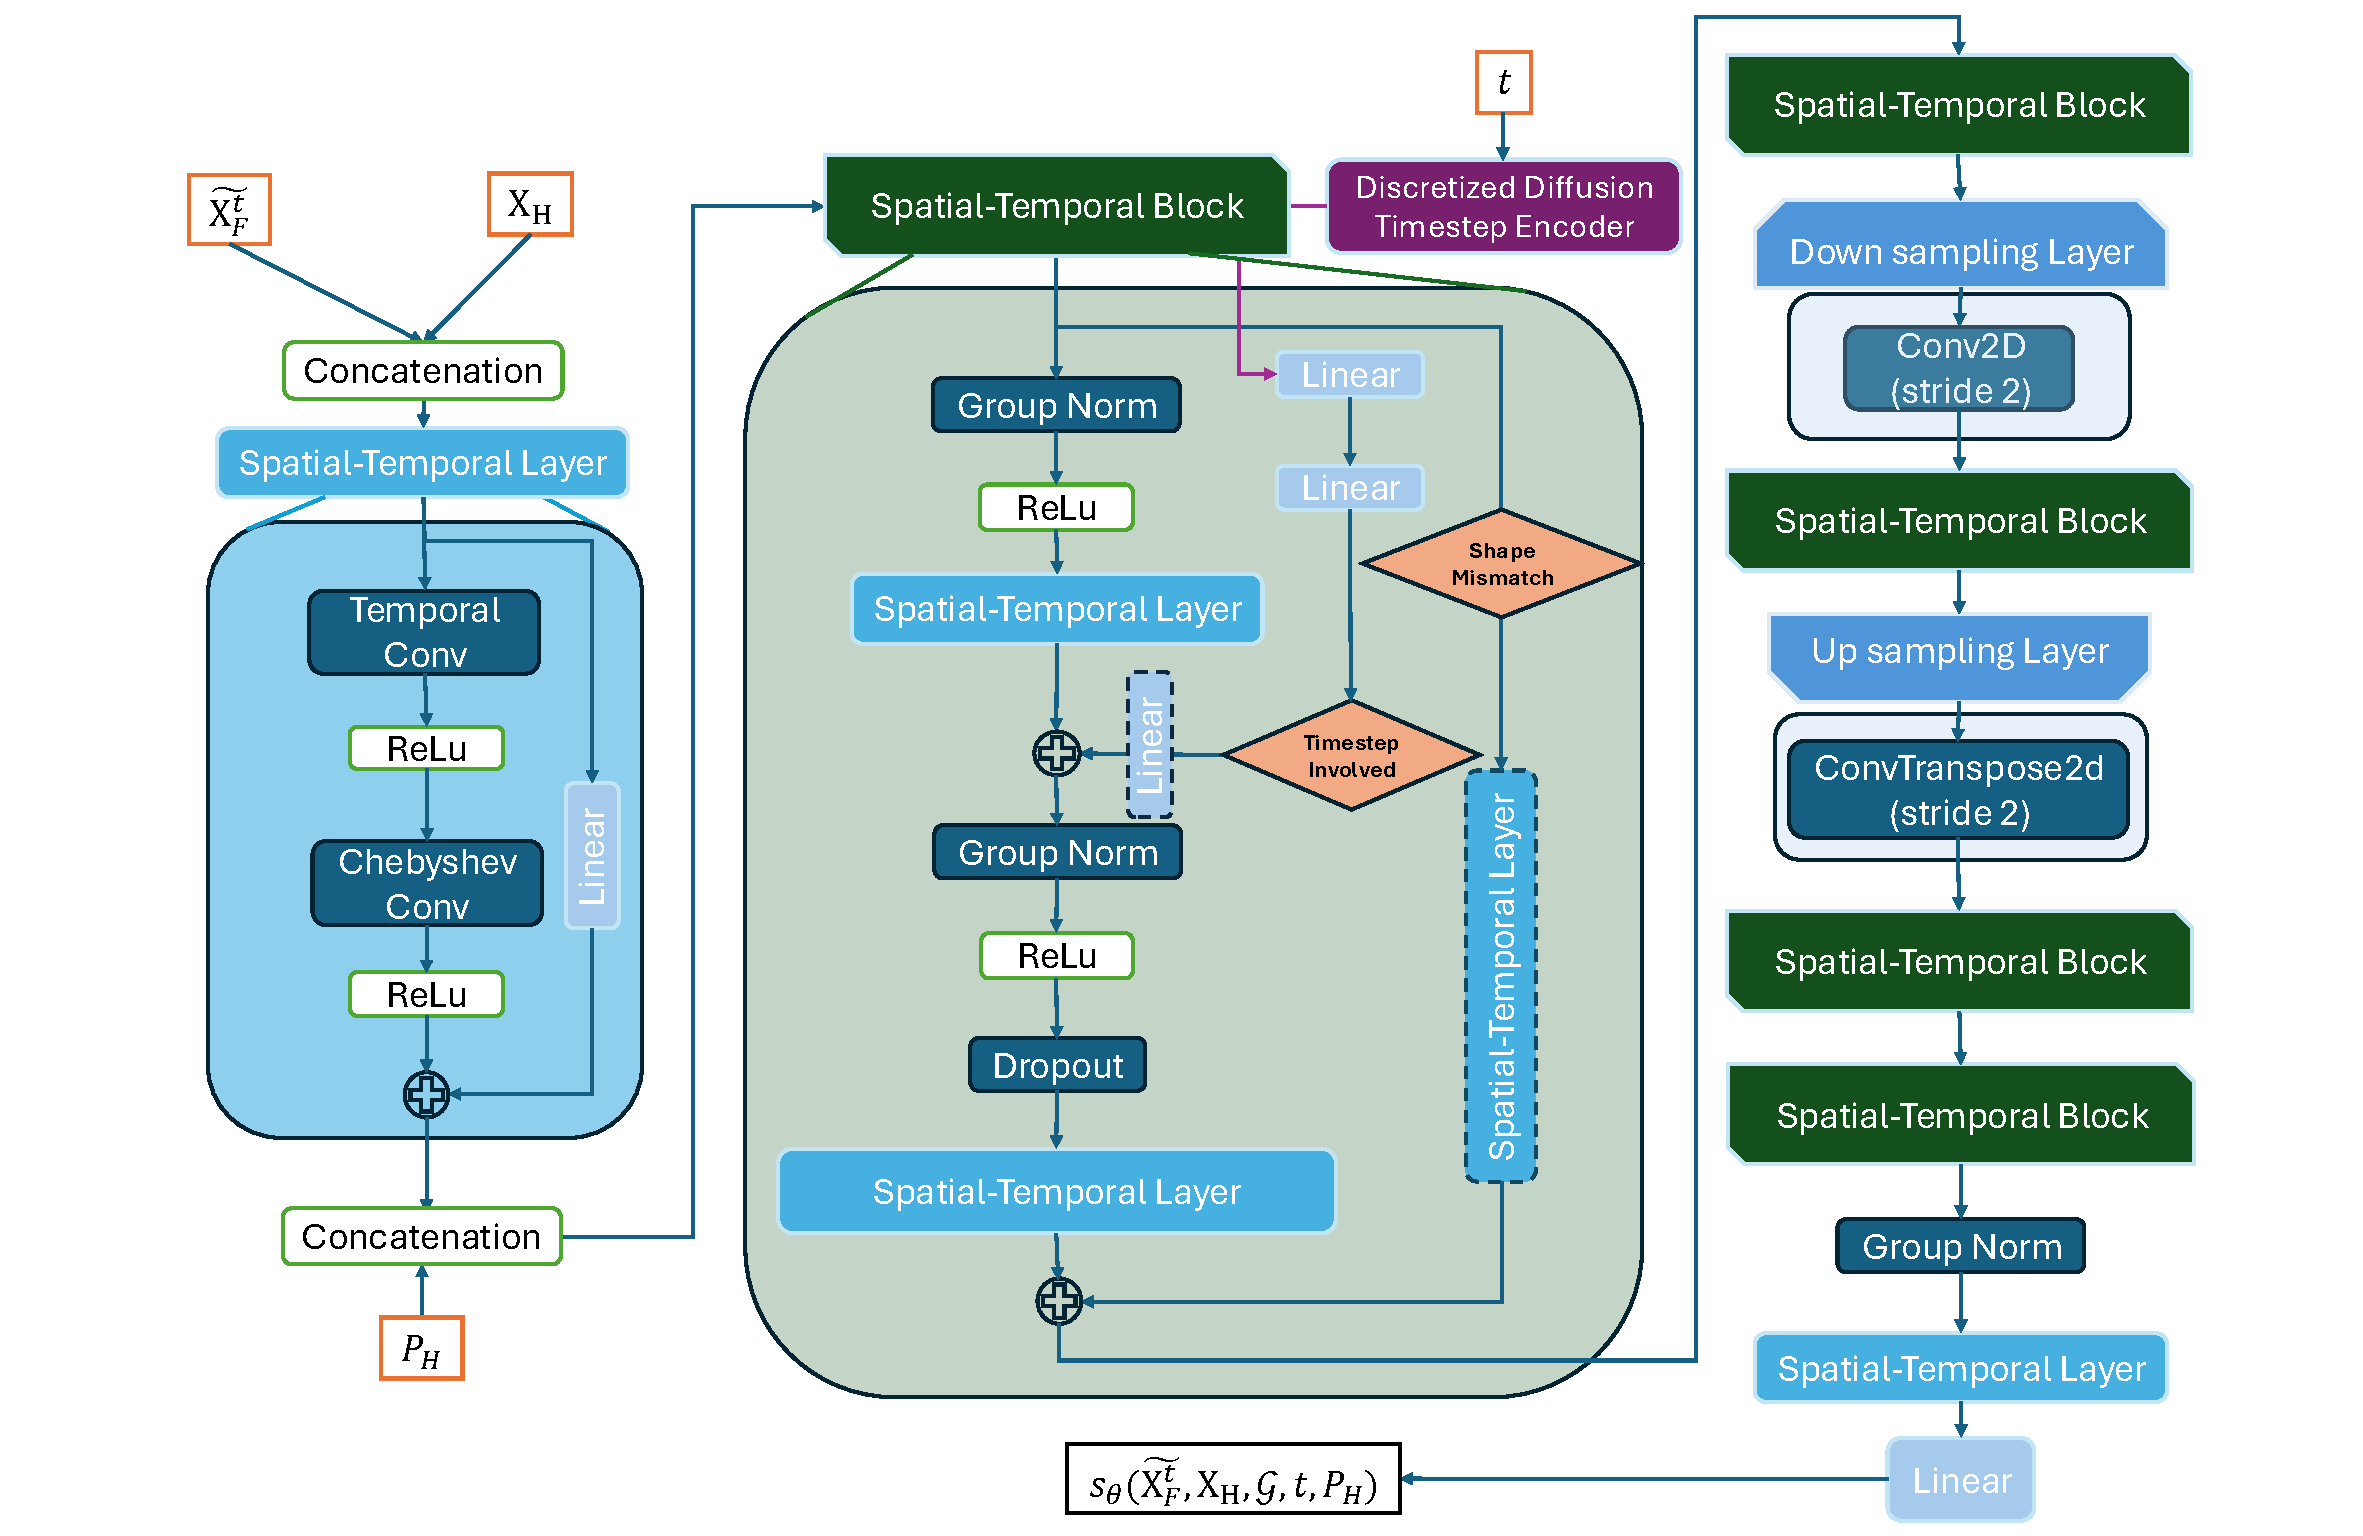
\includegraphics[width=0.7\textwidth]{figures/ProGen_model.pdf}
        \vspace{-0.7em}
        \caption{Architecture of the Denoising Score Matching Model in ProGen.}
        \label{fig:model}
    \end{figure}
\end{frame}


\begin{frame}
    \frametitle{Methodology}
    \framesubtitle{Adaptive Reverse Prediction Process}
    A new Spatial-Temporal SDE (ST SDE) is introduced to guide the reverse diffusion process:
    \begin{equation}
        \begin{aligned}
            d\mathbf{X} & = -\frac{1}{2} \beta(t)\left( \mathbf{X} - \alpha A \mathbf{X} \right)dt + \sqrt{\beta(t)(1 - e^{-2 \int_0^t \beta(s) \, ds})} \, dw,
        \end{aligned}
        \label{eq:spatiotemporal_sde}
    \end{equation}

    The reverse SDE effectively restores data from its noisy state using learned scores:
    \vspace{-0.4em}
    \begin{equation}
        \begin{aligned}
            \tilde{\mathbf{X}}_{\mathbf{F}}^{t - \frac{1}{K}} & = \tilde{\mathbf{X}}_{\mathbf{F}}^{t} - \left[ -\frac{1}{2} \beta(t) \left( \tilde{\mathbf{X}}_{\mathbf{F}}^{t} - \alpha A \tilde{\mathbf{X}}_{\mathbf{F}}^{t} \right) \, dt \right. \\
                                                              & \quad \left. - \left(\sqrt{\beta(t)(1 - e^{-2 \int_0^{t} \beta(s) \, ds})} \right)^2 \times s_\theta \right]                                                                         \\
                                                              & \quad + \sqrt{\beta(t)(1 - e^{-2 \int_0^{t} \beta(s) \, ds})} \cdot dW,
        \end{aligned}
        \label{eq:reverse_stdse}
    \end{equation}
    % This equation integrates insights from the score model to reverse the diffusion, guiding the data back to its original state. \\~\\

    % ProGen's approach modifies traditional methods by adapting to data dynamics more effectively and efficiently.
\end{frame}

\subsection{Results}
\begin{frame}
    \frametitle{Results}
    \framesubtitle{Overview of ProGen Performance on Full Test Runs}

    \begin{figure}[ht]
        \centering
        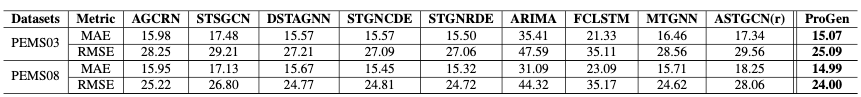
\includegraphics[width=\textwidth]{figures/det_full_tab.png}
        \caption{Deterministic performance on full PEMS03 and PEMS08 datasets.}
    \end{figure}

    \begin{figure}[htbp]
        \centering
        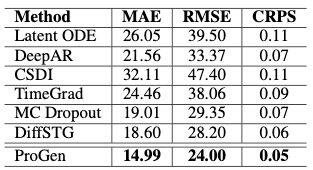
\includegraphics[width=0.35\textwidth]{figures/prob_full_tab.png}
        \caption{Probabilistic performance on full PEMS08 dataset.}
    \end{figure}
\end{frame}

\begin{frame}
    \frametitle{Results}
    \framesubtitle{Random Test Runs}

    \begin{figure}[ht]
        \centering
        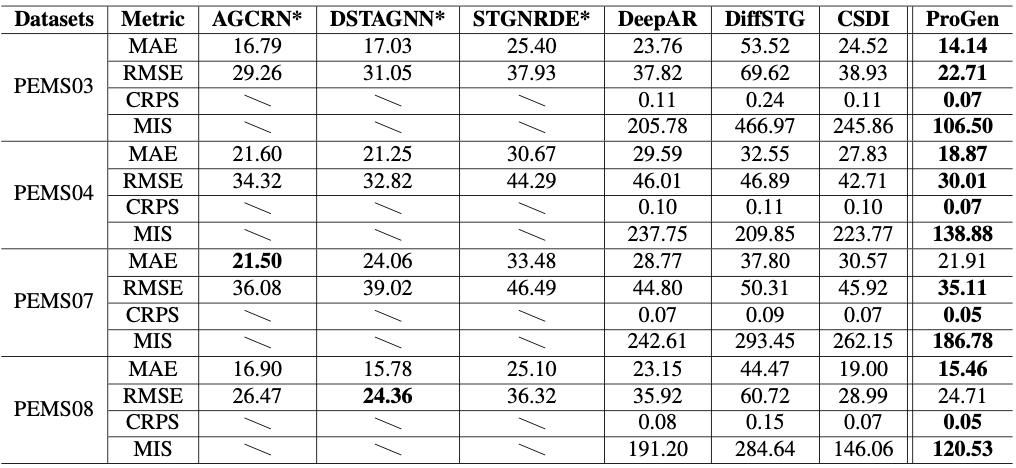
\includegraphics[width=0.8\textwidth]{figures/random_runs_tab.png}
        \caption{Overall performance on all datasets.}
    \end{figure}
\end{frame}


\begin{frame}
    \frametitle{Results}
    \framesubtitle{Generating Process Visualization}

    \begin{figure}[ht]
        \centering
        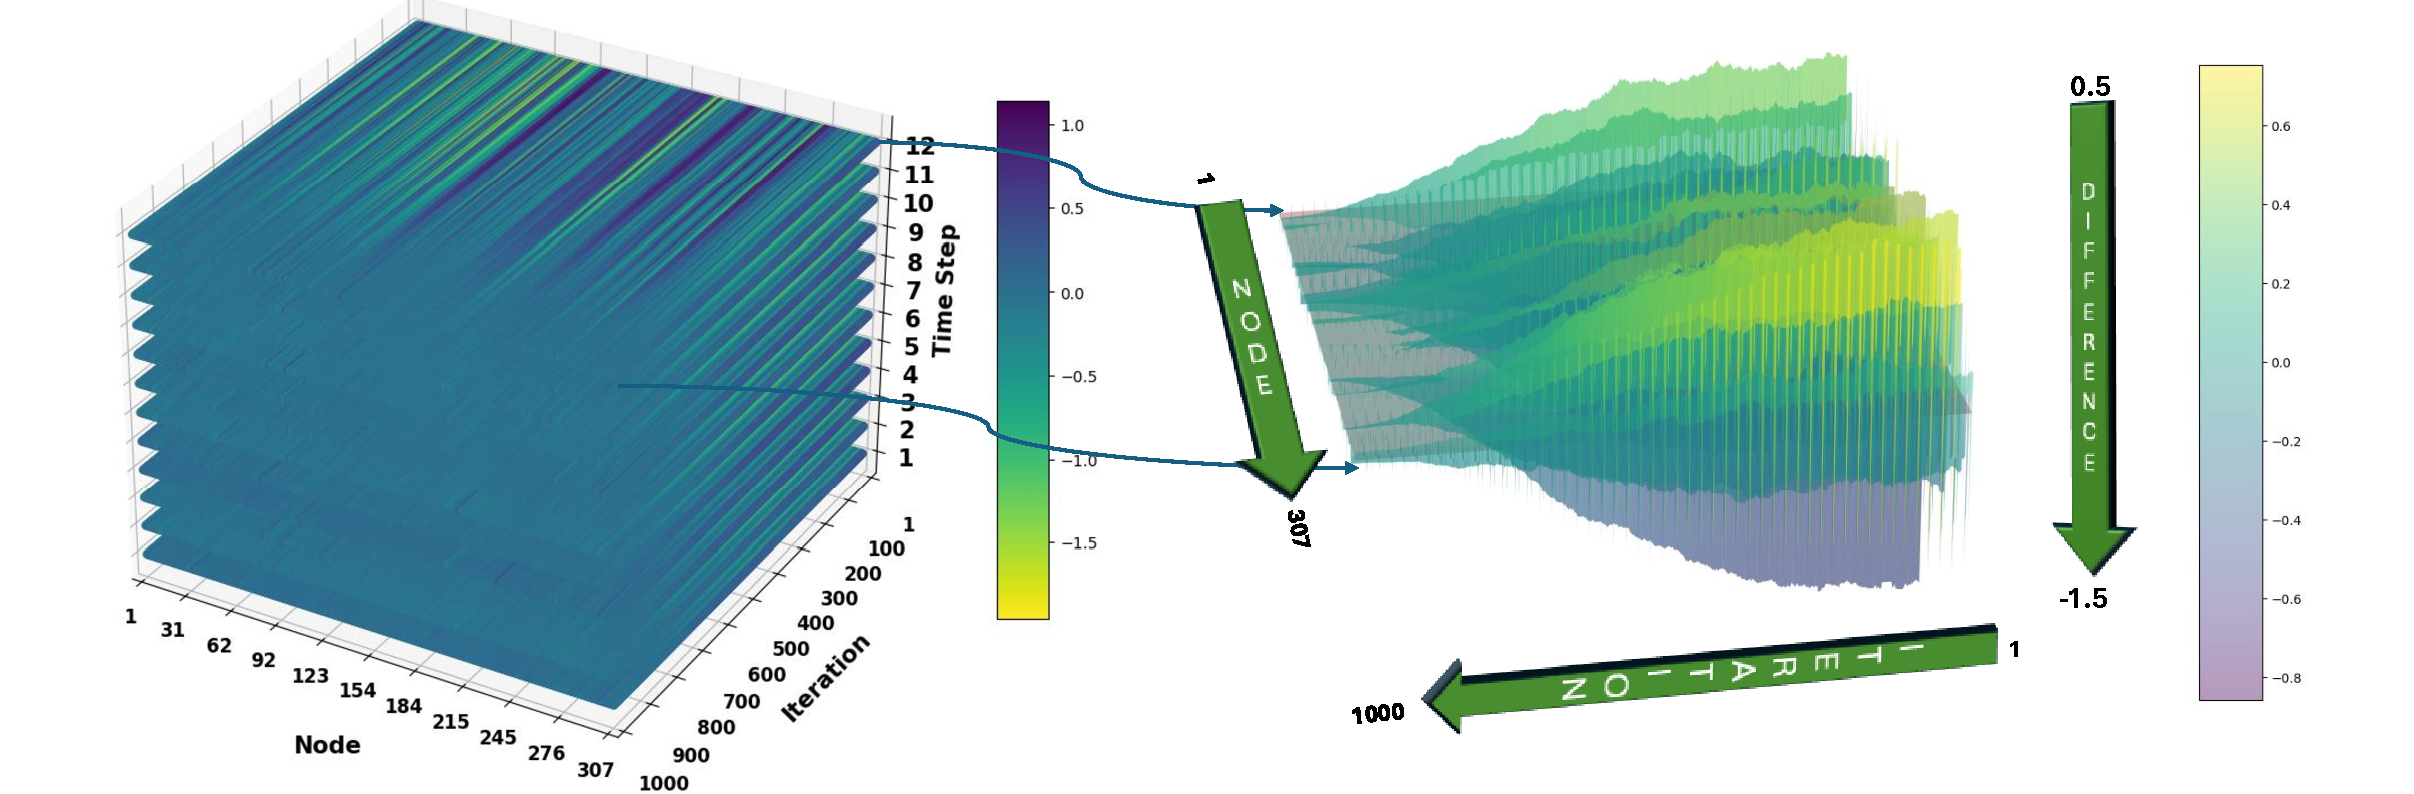
\includegraphics[width=\textwidth]{figures/pems04_3d_waves_plot.pdf}
        \caption{Visualization of the difference between the mean predictions and the actual values for the average test data in PEMS04.}
    \end{figure}
\end{frame}



\begin{frame}
    \frametitle{Results}
    \framesubtitle{Generating Process Visualization}

    \begin{figure}[ht]
        \centering
        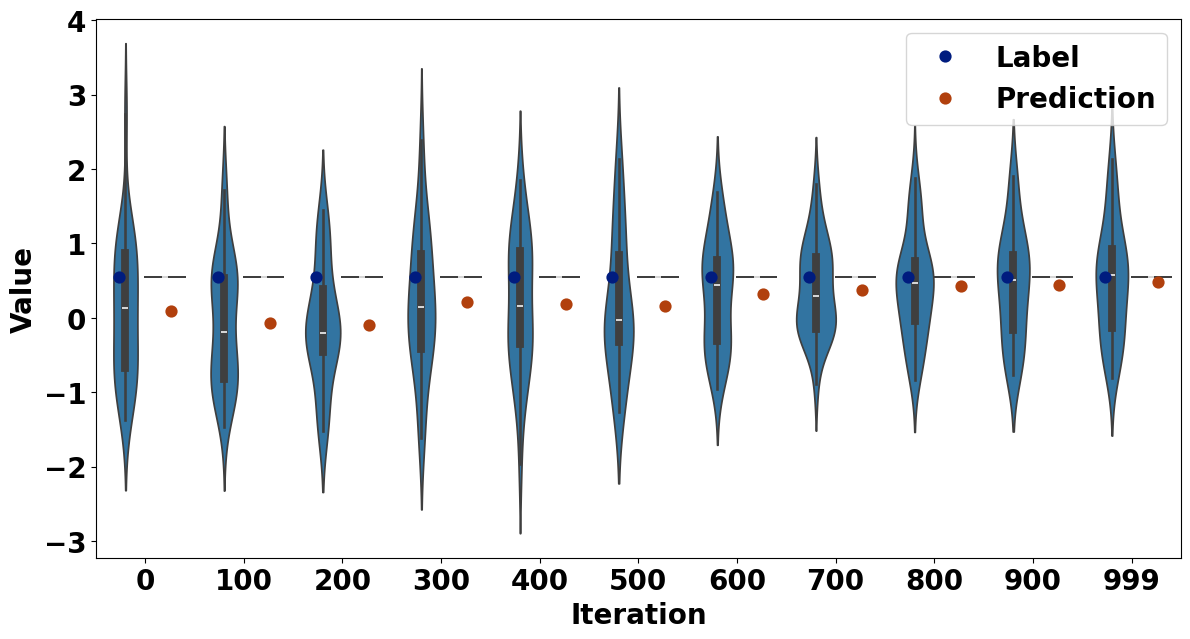
\includegraphics[width=0.8\textwidth]{figures/distribution_change_iteration_pems04.png}
        \vspace{-1em}
        \caption{Distribution and mean values of predictions vs. actual truths in PEMS04.}
    \end{figure}
\end{frame}


\begin{frame}
    \frametitle{Results}
    \framesubtitle{Ablation Studies}

    \begin{figure}[ht]
        \centering
        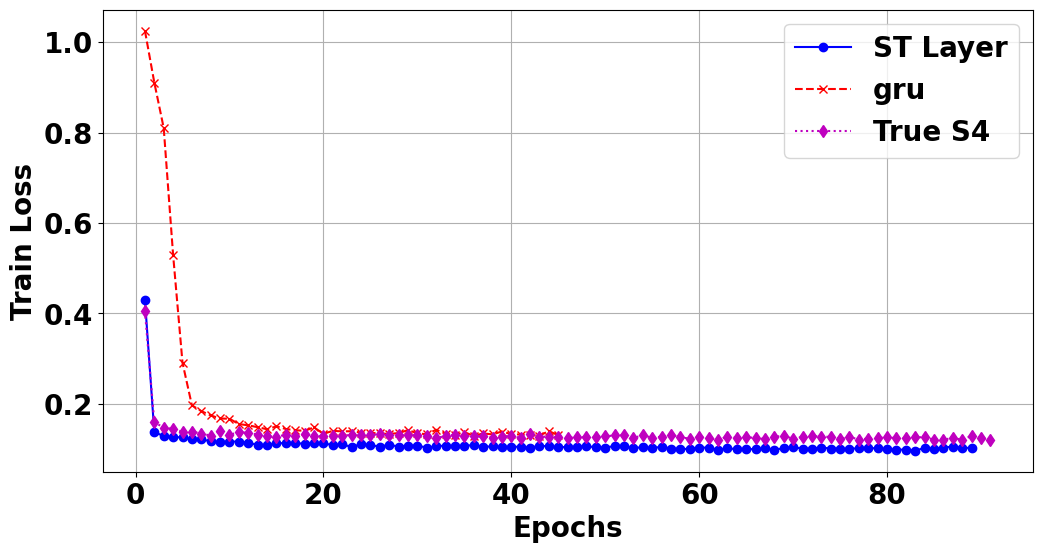
\includegraphics[width=0.8\textwidth]{figures/train_loss.png}
        \caption{Training loss curves for different spatiotemporal layers in PEMS08.}
    \end{figure}
\end{frame}

\begin{frame}
    \frametitle{Results}
    \framesubtitle{Ablation Studies}

    \begin{columns}
        \begin{column}{0.5\textwidth}
            \begin{figure}
                \centering
                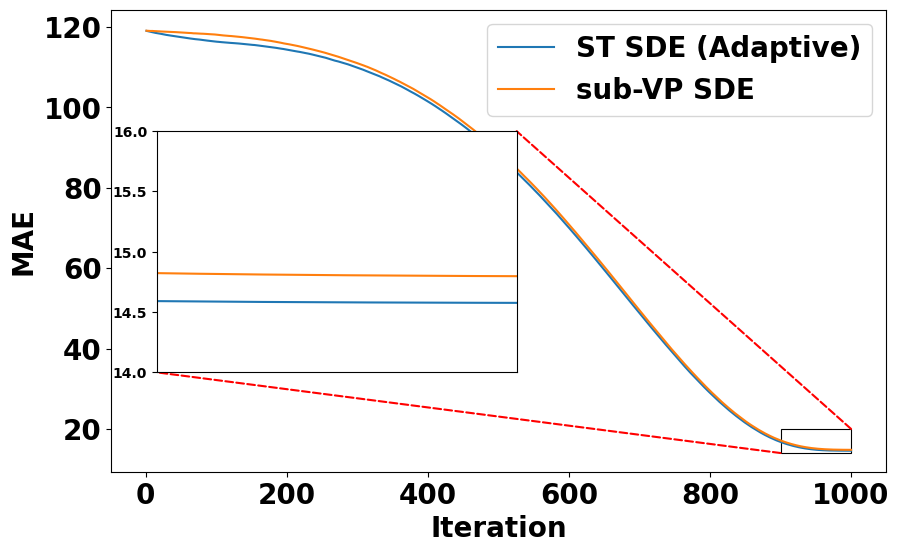
\includegraphics[width=\textwidth]{figures/mae_stsde_subvpsde.png}
                \caption{MAE comparison between the tailored spatial-temporal SDE and the subVP-SDE in PEMS08.}
            \end{figure}
        \end{column}
        \begin{column}{0.5\textwidth}
            \begin{figure}
                \centering
                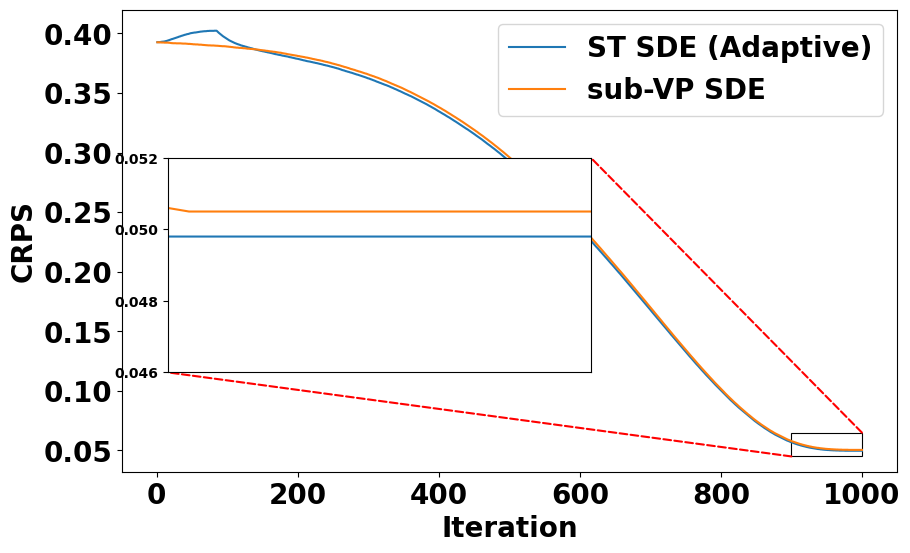
\includegraphics[width=\textwidth]{figures/crps_stsde_subvpsde.png}
                \caption{CRPS comparison between the tailored spatial-temporal SDE and the subVP-SDE in PEMS08.}
            \end{figure}
        \end{column}
    \end{columns}
\end{frame}

\begin{frame}
    \frametitle{Results}
    \framesubtitle{Ablation Studies}

    \begin{columns}
        \begin{column}{0.5\textwidth}
            \begin{figure}
                \centering
                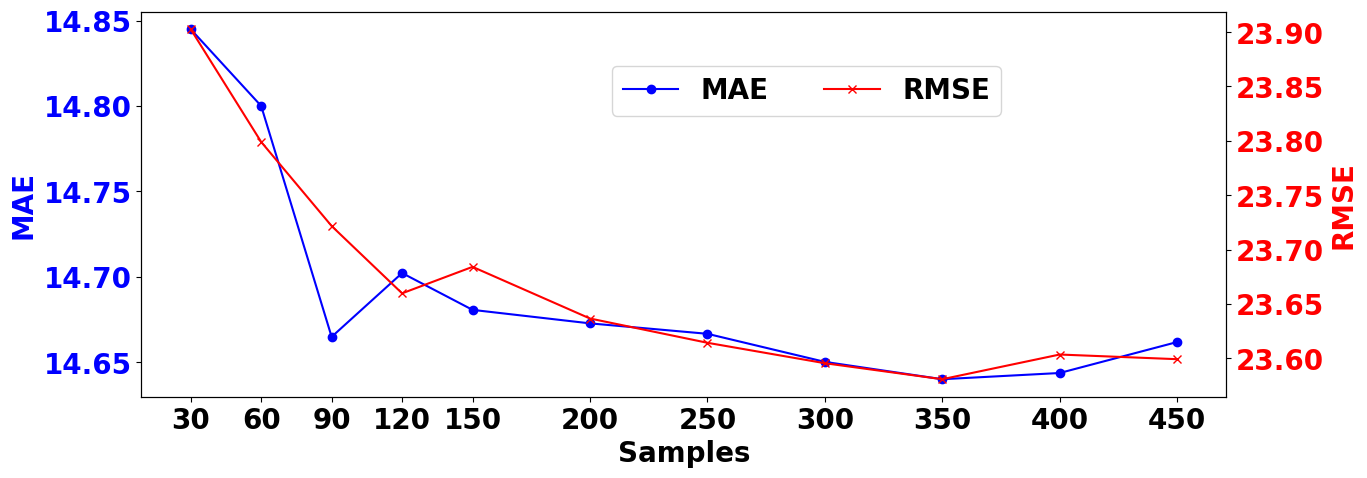
\includegraphics[width=\textwidth]{figures/mae_rmse_samples.png}
                \caption{MAE and RMSE across initial batch iterations in PEMS04.}
            \end{figure}
        \end{column}
        \begin{column}{0.5\textwidth}
            \begin{figure}
                \centering
                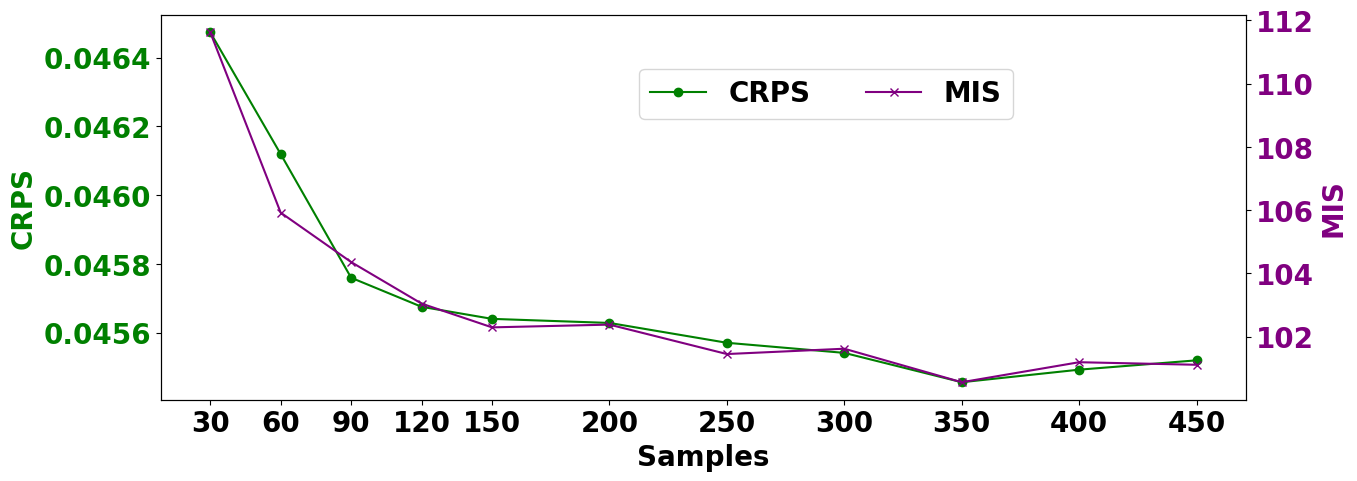
\includegraphics[width=\textwidth]{figures/crps_mis_samples.png}
                \caption{CRPS and MIS across initial batch iterations in PEMS04.}
            \end{figure}
        \end{column}
    \end{columns}

\end{frame}

\begin{frame}
    \frametitle{Results}
    \framesubtitle{Ablation Studies}
    \begin{columns}
        \begin{column}{0.5\textwidth}
            \begin{figure}
                \centering
                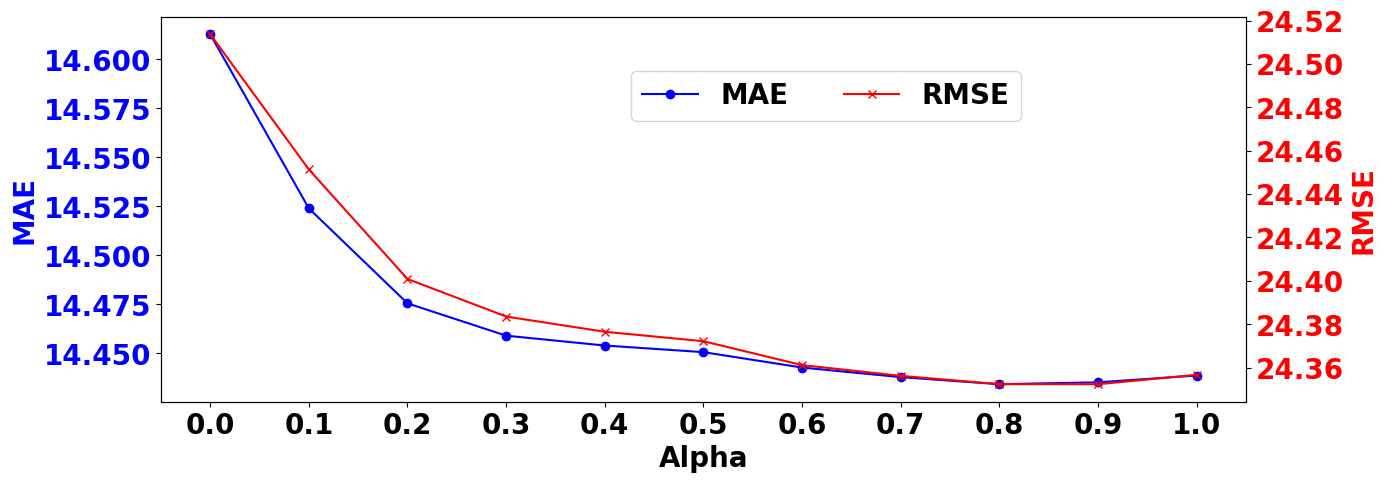
\includegraphics[width=\textwidth]{figures/pems07_mae_rmse_alpha.png}
                \caption{MAE and RMSE across initial batch iterations in PEMS04.}
            \end{figure}
        \end{column}
        \begin{column}{0.5\textwidth}
            \begin{figure}
                \centering
                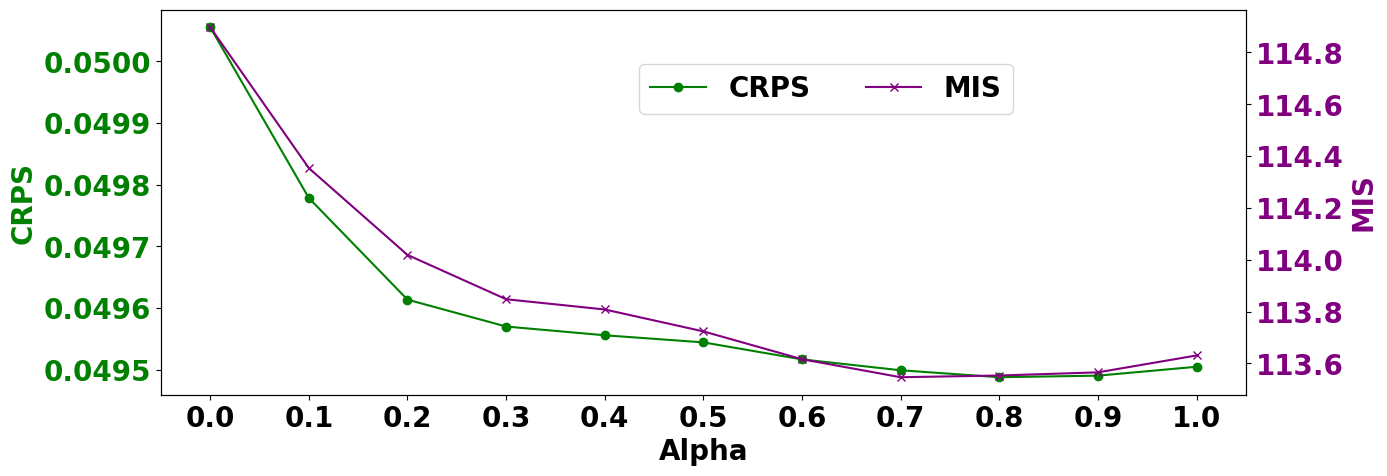
\includegraphics[width=\textwidth]{figures/pems07_crps_mis_alpha.png}
                \caption{CRPS and Miss Rate across initial batch iterations in PEMS04.}
            \end{figure}
        \end{column}
    \end{columns}

\end{frame}


% % % % % % % % % % % % % % % % % % % % % % % % % % % % % % % % % % % %
% % % % % % % % % % % % % % % % % % % % % % % % % % % % % % % % % % % %
% % % % % % % % % % % % % % % % % % % % % % % % % % % % % % % % % % % %
% % % % % % % % % % % % % % % % % % % % % % % % % % % % % % % % % % % %
% % % % % % % % % % % % % % % % % % % % % % % % % % % % % % % % % % % %
% % % % % % % % % % % % % % % % % % % % % % % % % % % % % % % % % % % %
% % % % % % % % % % % % % % % % % % % % % % % % % % % % % % % % % % % %
% % % % % % % % % % % % % % % % % % % % % % % % % % % % % % % % % % % %

\appendix % to start a separate page numbering

\section*{Bibliography}
\begin{frame}[allowframebreaks]
    \textbf{References}
    \printbibliography
\end{frame}


{ % all template changes are local to this group.
\setbeamertemplate{navigation symbols}{}
\begin{frame}<article:0>[plain,noframenumbering]
    \begin{tikzpicture}[remember picture,overlay]
        \node[at=(current page.center)] {
            
\includegraphics[
                width=\paperwidth,
                height=\paperheight]{figures/ThankYouPage.png}
        };
    \end{tikzpicture}
    % \begin{tikzpicture}[remember picture,overlay]
    %     \node[at=(current page.center)] {
    %         
\includegraphics[keepaspectratio,
    %             width=0.65\paperwidth,
    %             height=\paperheight]{figures/ThankYouPage.png}
    %     };
    % \end{tikzpicture}
\end{frame}
}

\end{document}
